\section{Quotient Groups and Homomorphisms}

\subsection{Definitions and Examples}

Let $G$ and $H$ be groups.

\begin{exercise}
    Let $\phi : G \to H$ be a homomorphism and let $E$ be a subgroup of $H$. Prove that $\phi\inv(E) \leq G$ (i.e., the preimage or pullback of a subgroup under a homomorphism is a subgroup). If $E \nsub H$ prove that $\phi\inv(E) \nsub G$. Deduce that $\ker(\phi) \nsub G$.
\end{exercise}

\begin{sol}
    Observe that $1_H \in E$. Since $\phi(1_G) = 1_H$, then $1_G \in \phi\inv(E)$ so that $\phi\inv(E)$ is nonempty. Let $x, y \in \phi\inv(E)$. Then $\phi(x), \phi(y) \in E$, so that $\phi(xy\inv) = \phi(x)\phi(y)\inv \in E$ since $E$ is a subgroup. Hence, $xy\inv \in \phi\inv(E)$ and $\phi\inv(E) \leq G$.

    Suppose $E \nsub H$. For any $h \in H$ and $e \in E$, then $heh\inv \in E$. Let $x \in \phi\inv(E)$ and $g \in G$. Then $\phi(x) \in E$ and $\phi(g) \in H$, so that
    \[\phi(gxg\inv) = \phi(g)\phi(x)\phi(g)\inv \in E\]
    and $gxg\inv \in \phi\inv(E)$. Hence, $\phi\inv(E) \nsub G$. Since $\ker\phi = \phi\inv(1_G)$, then $\ker\phi \nsub G$.
\end{sol}

\begin{exercise}
    Let $\varphi : G \to H$ be a homomorphism of groups with kernel $K$ and let $a,b \in \varphi(G)$. Let $X \in G/K$ be the fiber above $a$ and let $Y$ be the fiber above $b$, i.e., $X = \varphi^{-1}(a)$, $Y = \varphi^{-1}(b)$. Fix an element $u \in X$ (so $\varphi(u)=a$). Prove that if $XY = Z$ in the quotient group $G/K$ and $w$ is any member of $Z$, then there is some $v \in Y$ such that $uv = w$. [Show $u^{-1}w \in Y$.]
\end{exercise}

\begin{sol}
    Let $w \in Z$, and define $v = u\inv w$. Then
    \[\phi(v) = \phi(u\inv w) = \phi(u)\inv \phi(w) = a\inv (ab) = b\]
    so that $v \in Y$ and $uv = w$.
\end{sol}

\begin{exercise}
    Let $A$ be an abelian group and let $B$ be a subgroup of $A$. Prove that $A/B$ is abelian. Give an example of a non-abelian group $G$ containing a proper normal subgroup $N$ such that $G/N$ is abelian.
\end{exercise}

\begin{sol}
    Let $aB, a'B \in A/B$. Then
    \[(aB)(a'B) = (aa')B = (a'a)B = (a'B)(aB)\]
    so that $A/B$ is abelian.

    To produce an abelian quotient group from a non-abelian group, a good thought is to consider the centers of non-abelian groups. In this case, we may choose $G = D_8$ with $Z(D_8) = \gen{r^2} \nsub D_8$. Since $D_8/\gen{r^2} \cong V_4$, then the quotient group is abelian.
\end{sol}

\begin{exercise}
    Prove that in the quotient group $G/N$, $(gN)^{\alpha} = g^{\alpha}N$ for all $\alpha \in \mathbb{Z}$.
\end{exercise}

\begin{sol}
    We proceed by induction on $\alpha$. For the $\alpha = 0$ and $\alpha = -1$, observe that $(gN)^0 = 1N = g^0N$ by definition, and $(gN)\inv = g\inv N$ by Proposition 3.5. The base case of $\alpha = 1$ is trivial. Suppose that the relationship holds for some $\alpha \geq 1$. Then
    \[(gN)^{\alpha + 1} = (gN)^{\alpha}(gN) = (g^{\alpha}N)(gN) = g^{\alpha + 1}N\]
    so that the result is true by induction for all positive integers. For negative integers, use the result for positive integers along with the $\alpha = -1$ case.
\end{sol}

\begin{exercise}
    Use the preceding exercise to prove that the order of the element $gN$ in $G/N$ is $n$, where $n$ is the smallest positive integer such that $g^n \in N$ (and $gN$ has infinite order if no such positive integer exists). Give an example to show that the order of $gN$ in $G/N$ may be strictly smaller than the order of $g$ in $G$.
\end{exercise}

\begin{sol}
    Let $gN \in G/N$. If there exists some positive integer $n$ such that $g^n \in N$, then by the previous exercise, $(gN)^n = g^n N = N$ so that $|gN| \leq n$. If $|gN| = m$, then $g^mN = (gN)^m = N$, and $g^m \in N$. By the minimality of $n$, then $n \leq m$ so that $|gN| = n$.

    If there is no such $n$, then for every $m \in \zp$, we have that $g^m \not\in N$. Assume, by way of contradiction, that $|gN| = k$ for some $k \in \zp$. Then $g^kN = (gN)^k = N$, so that $g^k \in N$, a contradiction. Hence, $gN$ has infinite order.

    For an example, let $Z_4 = \gen x$. Then $|x| = 4$. Let $N = \gen{x^2}$. Then $N \nsub Z_4$ since $Z_4$ is abelian. However, $|xN| = 2$ since $(xN)^2 = x^2N = N$.
\end{sol}

\begin{exercise}
    Define $\varphi : \mathbb{R}^{\times} \to \{\pm 1\}$ by letting $\varphi(x)$ be $x$ divided by the absolute value of $x$. Describe the fibers of $\varphi$ and prove that $\varphi$ is a homomorphism.
\end{exercise}

\begin{sol}
    The fibers of $\phi$ are as follows: the positive reals map to 1, and the negative reals map to $-1$. Moreover, for any $x, y \in \r\unt$, then
    \[\phi(xy) = \frac{xy}{\abs{xy}} = \frac{x}{\abs x} \cdot \frac{y}{\abs y} = \phi(x)\phi(y) \qh\]
\end{sol}

\begin{exercise}
    Define $\pi : \mathbb{R}^2 \to \mathbb{R}$ by $\pi((x,y)) = x + y$. Prove that $\pi$ is a surjective homomorphism and describe the kernel and fibers of $\pi$ geometrically.
\end{exercise}

\begin{sol}
    Let $(x_1, y_1), (x_2, y_2) \in \r^2$. Then
    \begin{align*}
        \pi((x_1, y_1) + (x_2, y_2)) & = \pi((x_1 + x_2, y_1 + y_2)) \\
        & = (x_1 + x_2) + (y_1 + y_2) \\
        & = (x_1 + y_1) + (x_2 + y_2) \\
        & = \pi((x_1, y_1)) + \pi((x_2, y_2))
    \end{align*}
    so that $\pi$ is a homomorphism. Moreover, $\pi((a, 0)) = a$ for any $a \in \r$, so $\pi$ is surjective. $\ker\pi$ is the line $y = -x$ in the plane, and the fiber $\pi\inv(a)$ for any $a \in \r$ is the line $y = a - x$, or the vertical translation of $\ker\pi$ by $a$ units.
\end{sol}

\begin{exercise}
    Let $\varphi : \mathbb{R}^{\times} \to \mathbb{R}^{\times}$ be the map sending $x$ to the absolute value of $x$. Prove that $\varphi$ is a homomorphism and find the image of $\varphi$. Describe the kernel and the fibers of $\varphi$.
\end{exercise}

\begin{sol}
    Let $x, y \in \r\unt$. Then
    \[\phi(xy) = \abs{xy} = \abs x \abs y = \phi(x)\phi(y)\]
    so that $\phi$ is a homomorphism. Note that $\abs x > 0$ for any $x \in \r\unt$, so $\im(\phi) = \r^+$. $\ker(\phi) = \{-1, 1\}$, and the fiber of $\phi$ over some $a \in \r^+$ is simply $\{-a, a\}$.
\end{sol}

\newpage

\begin{exercise}
    Define $\varphi : \mathbb{C}^{\times} \to \mathbb{R}^{\times}$ by $\varphi(a+bi) = a^2 + b^2$. Prove that $\varphi$ is a homomorphism and find the image of $\varphi$. Describe the kernel and the fibers of $\varphi$ geometrically (as subsets of the plane).
\end{exercise}

\begin{sol}
    Let $a + bi, c + di \in \c\unt$. Then
    \begin{align*}
        \phi((a + bi)(c + di)) & = \phi((ac - bd) + (ad + bc)i) \\
        & = (ac - bd)^2 + (ad + bc)^2 \\
        & = a^2c^2 - 2abcd + b^2d^2 + a^2d^2 + 2abcd + b^2c^2 \\
        & = c^2(a^2 + b^2) + d^2(a^2 + b^2) \\
        & = (a^2 + b^2)(c^2 + d^2) \\
        & = \phi(a + bi)\phi(c + di)
    \end{align*}
    so that $\phi$ is a homomorphism. Observe that $a^2 + b^2 > 0$ for any $a + bi \in \c\unt$, so that $\im(\phi) = \r^+$. $\ker\phi$ is the unit circle in the complex plane, and the fiber of $\phi$ over some $r \in \r^+$ is the circle of radius $\sqrt r$ centered at the origin.
\end{sol}

\begin{exercise}
    Let $\phi : \intmod[8] \to \intmod[4]$ by $\phi(\bar  a) = \bar  a$. Show that this is a well defined, surjective homomorphism and describe its fibers and kernel explicitly (showing that $\phi$ is well defined involves the fact that $\bar  a$ has a different meaning in the domain and range of $\phi$).
\end{exercise}

\begin{sol}
    To show that $\phi$ is well-defined, suppose $\bar a = \bar b$ in $\intmod[8]$. Then $8 \mid (a - b)$, so that $a - b = 8k$ for some $k \in \z$. Then $a - b = 4(2k)$, so that $4 \mid (a - b)$ and $\bar a = \bar b$ in $\intmod[4]$. Hence, $\phi$ is well-defined. Moreover, for any $\bar a, \bar b \in \intmod[8]$, then
    \[\phi(\bar a + \bar b) = \phi(\overline{a + b}) = \overline{a + b} = \bar a + \bar b = \phi(\bar a) + \phi(\bar b)\]
    so that $\phi$ is a homomorphism. Note that for any $\bar c \in \intmod[4]$, then $\phi(\bar c) = \bar c$, so $\phi$ is surjective. The fibers of $\phi$:
    \begin{align*}
        \phi\inv(\bar 0) & = \{\bar 0, \bar 4\} \\
        \phi\inv(\bar 1) & = \{\bar 1, \bar 5\} \\
        \phi\inv(\bar 2) & = \{\bar 2, \bar 6\} \\
        \phi\inv(\bar 3) & = \{\bar 3, \bar 7\}
    \end{align*}
    with $\ker\phi = \phi\inv(\bar 0) = \{\bar 0, \bar 4\}$.
\end{sol}

\begin{exercise}
    Let $F$ be a field and let
    \[G = \set*{\left.
    \begin{pmatrix}
        a & b \\
        0 & c 
    \end{pmatrix}~\right|~a, b, c \in F, ac \neq 0} \leq \gl_2(F)\]
    \begin{subproblems}
        \item Prove that the map
        \[\phi : 
        \begin{pmatrix}
            a & b \\
            0 & c
        \end{pmatrix} \mapsto a\]
        is a surjective homomorphism from $G$ onto $F\unt$ (recall that $F\unt$ is the multiplicative group of nonzero elements in $F$). Describe the fibers and kernel of $\phi$.
        \item Prove that the map
        \[\psi : 
        \begin{pmatrix}
            a & b \\
            0 & c
        \end{pmatrix} \mapsto (a, c)\]
        is a surjective homomorphism from $G$ onto $F\unt \times F\unt$. Describe the fibers and kernel of $\psi$. 
        \item Let
        \[H = \set*{\left .
        \begin{pmatrix}
            1 & b \\
            0 & 1
        \end{pmatrix} ~\right\vert~b \in F}\]
        Prove that $H$ is isomorphic to the additive group $F$.
    \end{subproblems}
\end{exercise}

\begin{solalph}
    \item Observe that
    \[\phi\left(
    \begin{pmatrix}
        a & 1 \\
        0 & 1
    \end{pmatrix}\right) = a\]
    so that $\phi$ is surjective. Moreover, for any $a, b, c, d, e, f \in F$ with $ac \neq 0$ and $df \neq 0$, we have
    \[\phi\left(
    \begin{pmatrix}
        a & b \\
        0 & c
    \end{pmatrix}
    \begin{pmatrix}
        d & e \\
        0 & f
    \end{pmatrix}\right) = 
    \phi\left(
    \begin{pmatrix}
        ad & ae + bf \\
        0 & cf
    \end{pmatrix}\right) = ad = 
    \phi\left(
    \begin{pmatrix}
        a & b \\
        0 & c
    \end{pmatrix}\right)
    \phi\left(
    \begin{pmatrix}
        d & e \\
        0 & f
    \end{pmatrix}\right)\]
    and $\phi$ is then a homomorphism. The fiber of $a \in F\unt$ over $\phi$ is
    \[\phi\inv(a) = 
    \set*{\left.
    \begin{pmatrix}
        a & s \\
        0 & t
    \end{pmatrix}~\right|~s, t \in F, t \neq 0}\]
    with $\ker\phi = \phi\inv(1)$.
    \item To show that $\psi$ is surjective is similar as the previous exercise. The fiber of any $(a, c) \in F\unt \times F\unt$ is
    \[\psi\inv((a, c)) = 
    \set*{\left.
    \begin{pmatrix}
        a & s \\
        0 & c
    \end{pmatrix}~\right|~s \in F}\]
    with $\ker\psi = \psi\inv((1, 1))$.
    \item Define the mapping $\pi_1 : H \to F$ given by
    \[\pi_1\left(
    \begin{pmatrix}
        1 & b \\
        0 & 1
    \end{pmatrix}\right) = b\]
    Define another map $\pi_2 : F \to H$ given by
    \[\pi_2(b) = 
    \begin{pmatrix}
        1 & b \\
        0 & 1
    \end{pmatrix}\]
    It is clear that $\pi_2$ is a two-sided inverse of $\pi_1$. For any $b, c \in F$, we have
    \[\pi_1\left(
    \begin{pmatrix}
        1 & b \\
        0 & 1
    \end{pmatrix}
    \begin{pmatrix}
        1 & c \\
        0 & 1
    \end{pmatrix}\right) = 
    \pi_1\left(
    \begin{pmatrix}
        1 & b + c \\
        0 & 1
    \end{pmatrix}\right) = b + c = 
    \pi_1\left(
    \begin{pmatrix}
        1 & b \\
        0 & 1
    \end{pmatrix}\right) + 
    \pi_1\left(
    \begin{pmatrix}
        1 & c \\
        0 & 1
    \end{pmatrix}\right)\]
    so that $\pi_1$ is a homomorphism. Then $\pi_1$ is an isomorphism, and $H \cong F$.
\end{solalph}

\begin{exercise} \label{ex3.1.12}
    Let $G$ be the additive group of real numbers, let $H$ be the multiplicative group of complex numbers of absolute value $1$ (the unit circle $S^1$ in the complex plane) and let $\varphi : G \to H$ be the homomorphism $\varphi : r \mapsto e^{2\pi i r}$. Draw the points on a real line which lie in the kernel of $\varphi$. Describe similarly the elements in the fibers of $\varphi$ above the points $-1$, $i$, and $e^{4\pi i/3}$ of $H$.
\end{exercise}

\begin{sol}
    Since $e^{2\pi ir} = 1$ if and only if $r$ is an integer, then $\ker(\phi) = \z$. On a number line, this is shown as
    \begin{center}
        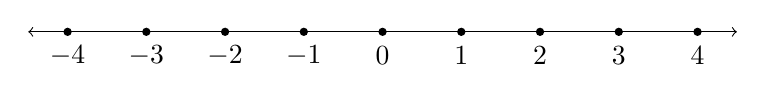
\begin{tikzpicture}
            \draw[<->] (-4.5, 0) -- (4.5, 0);

            \foreach \x in {-4, -3, -2, -1, 0, 1, 2, 3, 4}
                \fill (\x, 0) circle (1.5pt);

            \foreach \x in {-4, -3, -2, -1, 0, 1, 2, 3, 4}
                \node at (\x, -0.3) {$\x$};
        \end{tikzpicture}
    \end{center}
    Moreover, note that $-1 = e^{-2\pi i/2}$ and $i = e^{2\pi i/4}$. Then the fibers of these elements are just the integral differences of $1/2, 1/4$, and $2/3$ respectively, since $4\pi i/3 = 2/3(2\pi i)$:
    \begin{align*}
        \phi\inv(-1) & = \frac 12 + \z = \set*{\left.\frac 12 + n~\right|~n \in \z} \\
        \phi\inv(i) & = \frac 14 + \z = \set*{\left.\frac 14 + n~\right|~n \in \z} \\
        \phi\inv(e^{4\pi i/3}) & = \frac 23 + \z = \set*{\left.\frac 23 + n~\right|~n \in \z} \qh
    \end{align*}
\end{sol}

\begin{exercise}
    Repeat the preceding exercise with the map $\varphi$ replaced by the map $\varphi : r \mapsto e^{4\pi i r}$.
\end{exercise}

\begin{sol}
    The kernel of $\phi$ is $\frac12\z$, or
    \begin{center}
        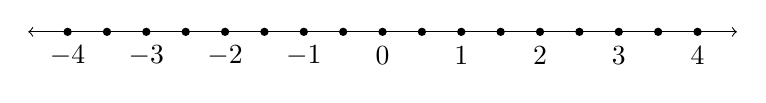
\begin{tikzpicture}
            \draw[<->] (-4.5, 0) -- (4.5, 0);

            \foreach \x in {-4, -3.5, -3, -2.5, -2, -1.5, -1, -0.5, 0, 0.5, 1, 1.5, 2, 2.5, 3, 3.5, 4}
                \fill (\x, 0) circle (1.5pt);

            \foreach \x in {-4, -3, -2, -1, 0, 1, 2, 3, 4}
                \node at (\x, -0.3) {$\x$};
        \end{tikzpicture}
    \end{center}
    Moreover, the fibers are just all halved, so
    \begin{align*}
        \phi\inv(-1) & = \frac14 + \frac12 \z = \set*{\left.\frac14 + \frac n2~\right|~n \in \z} \\
        \phi\inv(-i) & = \frac18 + \frac12 \z = \set*{\left.\frac18 + \frac n2~\right|~n \in \z} \\
        \phi\inv(e^{4\pi i/3}) & = \frac13 + \frac12 \z = \set*{\left.\frac13 + \frac n2~\right|~n \in \z} \qh
    \end{align*}
\end{sol}

\newpage

\begin{specialexercise}
    Consider the additive quotient group $\mathbb{Q}/\mathbb{Z}$.
    \begin{subproblems}
        \item Show that every coset of $\mathbb{Z}$ in $\mathbb{Q}$ contains exactly one representative $q \in \mathbb{Q}$ in the range $0 \le q < 1$.
        \item Show that every element of $\mathbb{Q}/\mathbb{Z}$ has finite order but that there are elements of arbitrarily large order.
        \item Show that $\mathbb{Q}/\mathbb{Z}$ is the torsion subgroup of $\mathbb{R}/\mathbb{Z}$ (cf. \hyperref[ex2.1.6]{Exercise 2.1.6}).
        \item Prove that $\mathbb{Q}/\mathbb{Z}$ is isomorphic to the multiplicative group of roots of unity in $\mathbb{C}^\times$.
    \end{subproblems}
\end{specialexercise}

\begin{solalph}
    \item Suppose $a/b \in \q$ with $(a, b) = 1$. By the Division Algorithm, there exist unique integers $q, r$ such that $a = bq + r$ for $0 \leq r < b$, or equivalently, $a/b = q + r/b$. Then $a/b + \z = r/b + \z$. If there exists some other representative $s/t$ in $0 \leq s/t < 1$ such that $a/b + \z = s/t + \z$, then $r/b + \z = s/t + \z$, or that $r/b - s/t \in \z$. Then there exists some integer $k$ such that $rt - sb = kbt$. Since $0 \leq r < b$ and $0 \leq s < t$, then $0 \leq rt < bt$ and $0 \leq sb < bt$. Combining these two inequalities, we get $-bt < rt - sb < bt$, so that $-1 < k < 1$. Since $k$ is an integer, then $k = 0$, and $rt - sb = 0$, or $r/b = s/t$. Hence, the representative in $0 \leq q < 1$ is unique.
    \item Let $a/b \in \q$. Then $b(a/b + \z) = ab + \z = \z$, so that $a/b + \z$ has finite order. Moreover, $1/k + \z \in \q/\z$ has order $k$, and since $k$ can be made arbitrarily large, then there are elements of arbitrarily large order.
    \item By the previous exercise, $\q/\z \subseteq \tor(\r/\z)$. Let $x + \z \in \tor(\r/\z)$. Then $|x + \z|$ is finite, so there exists some $n \in \z$ such that $n(x + \z) = nx + \z = \z$. Then $nx \in \z$, so that $x = m/n$ for some $m \in \z$. Hence, $x + \z \in \q/\z$, and $\tor(\r/\z) \subseteq \q/\z$. Therefore, $\tor(\r/\z) = \q/\z$.
    \item By \hyperref[ex3.1.12]{Exercise 3.1.12}, we have $\r/\z \cong S^1$. By definition, $\tor(S^1)$ consists of $z \in \c\unt$ such that $z^n = 1$ for some $n \in \zp$. This is precisely the set of roots of unity. Since $\tor(\r/\z) = \q/\z$, then $\q/\z$ is isomorphic to the set of roots of unity.
\end{solalph}

\begin{exercise}
    \label{ex3.1.15} Prove that a quotient of a divisible abelian group by any proper subgroup is also divisible. Deduce that $\mathbb{Q}/\mathbb{Z}$ is divisible (cf. \hyperref[ex2.4.19]{Exercise 2.4.19}).
\end{exercise}

\begin{sol}
    Since $A$ is abelian, any proper subgroup $B$ of $A$ is normal. To that end, let $aB \in A/B$, and let $n \in \zp$. Since $A$ is divisible, there exists some $x \in A$ such that $x^n = a$. Then
    \[(xB)^n = x^n B = aB\]
    so that $A/B$ is divisible. Observe that $\q$ is divisible, since for any $q \in \q$ and $n \in \zp$, there exists $p \in \q$ such that $np = q$, namely $p = q/n$. Moreover, $\z$ is a proper subgroup of $\q$, so by the first part, $\q/\z$ is divisible.
\end{sol}

\begin{specialexercise}
    Let $G$ be a group, let $N$ be a normal subgroup of $G$, and let $\bar{G} = G/N$. Prove that if $G = \langle x, y \rangle$ then $\bar{G} = \langle \bar{x}, \bar{y} \rangle$. Prove more generally that if $G = \langle S \rangle$ for any subset $S$ of $G$, then $\bar{G} = \langle \bar{S} \rangle$.
\end{specialexercise}

\begin{sol}
    We prove the general case. Since $G = \gen S$, then for any $g \in G$, we have
    \[g = s_1^{\alpha_1} s_2^{\alpha_2} \cdots s_k^{\alpha_k}, \quad s_i \in S, \alpha_i \in \z\]
    Observe that $\bar S = \{\bar s \mid s \in S\}$. Then for any $\bar g \in \bar G$, we have
    \[\bar g = \bar{s_1^{\alpha_1} s_2^{\alpha_2} \cdots s_k^{\alpha_k}} = \bar s_1^{\alpha_1} \bar s_2^{\alpha_2} \cdots \bar s_k^{\alpha_k}\]
    so that $\bar g \in \gen{\bar S}$. Hence, $\bar G \subseteq \gen{\bar S}$. Since $\bar s \in \bar G$ for any $s \in S$, then $\gen{\bar S} \subseteq \bar G$. Therefore, $\bar G = \gen{\bar S}$.

    The case of $G = \gen{x, y}$ is a special case where $S = \{x, y\}$.
\end{sol}

\begin{exercise}
    Let $G$ be the dihedral group of order $16$ (whose lattice appears in Section 2.5): $G = \langle r,s \mid r^8 = s^2 = 1,\ rs = sr^{-1} \rangle$, and let $\bar{G} = G/\langle r^4 \rangle$ be the quotient of $G$ by the subgroup generated by $r^4$ (this subgroup is the center of $G$, hence is normal).
    \begin{subproblems}
        \item Show that the order of $\bar{G}$ is $8$.
        \item Exhibit each element of $\bar{G}$ in the form $\bar{s}^a \bar{r}^b$, for some integers $a$ and $b$.
        \item Find the order of each of the elements of $\bar{G}$ exhibited in (b).
        \item Write each of the following elements of $\bar{G}$ in the form $\bar{s}^a \bar{r}^b$, for some integers $a$ and $b$ as in (b): $\bar{rs}$, $\bar{sr^{-2}s}$, $\bar{s^{-1}r^{-1}sr}$.
        \item Prove that $\bar{H} = \langle \bar{s}, \bar{r}^2 \rangle$ is a normal subgroup of $\bar{G}$ and $\bar{H}$ is isomorphic to the Klein $4$-group. Describe the isomorphism type of the complete preimage of $\bar{H}$ in $G$.
        \item Find the center of $\bar G$ and describe the isomorphism type of $\bar G/Z(\bar G)$.
    \end{subproblems}
\end{exercise}

\begin{solalph}
    \item Since $\gen{r^4} = \set{1, r^4}$, each coset in $\bar G$ has 2 elements and partitions $G$ into 8 sets. Hence, $\abs{\bar G} = 8$.
    \item The elements of $\bar G$ are
    \begin{align*}
        \bar 1 & = \{1, r^4\}, & \bar{s} & = \{s, sr^4\} \\
        \bar r & = \{r, r^5\}, & \bar{sr} & = \{sr, sr^5\} \\
        \bar r^2 & = \{r^2, r^6\}, & \bar{sr^2} & = \{sr^2, sr^6\} \\
        \bar r^3 & = \{r^3, r^7\}, & \bar{sr^3} & = \{sr^3, sr^7\}
    \end{align*}
    \item The orders of the elements of $\bar G$ are
    \[
    \begin{array}{c|c|c|c|c|c|c|c|c}
        \bar x & \bar 1 & \bar r & \bar r^2 & \bar r^3 & \bar s & \bar{sr} & \bar{sr^2} & \bar{sr^3} \\
        \hline
        \abs x & 1 & 4 & 2 & 4 & 2 & 2 & 2 & 2
    \end{array}
    \]
    \item $\bar{rs} = \bar{sr^3}, \bar{sr^{-2}s} = \bar r^2, \bar{s\inv r\inv sr} = \bar r^2$.
    \item We first note that $\bar H = \{1, \bar r^2, \bar s, \bar{sr^2}\}$. To show that $\bar H \nsub \bar G$, we simplify the process by noting that elements of $\bar G$ are of the form $\bar r^k$ or $\bar{sr^k}$. If an element is of the former, we have
    \begin{align*}
        \bar{r^kr^2r^{-k}} = \bar r^2 \in \bar H \\
        \bar{r^ksr^{-k}} = \bar{s(r^2)^{-k}} \in \bar H
    \end{align*}
    If it is of the latter, then
    \begin{align*}
        \bar{(sr^k)r^2(r^{-k}s)} = \bar{r^{-2}} \in H \\
        \bar{(sr^k)s(r^{-k}s)} = \bar{s(r^2)^k} \in H
    \end{align*}
    where $\bar{sr^k}\inv = \bar{r^{-k}s}$. The above calculations show that for every $\bar g \in \bar G$, then $\bar{gr^2g\inv}, \bar{gsg\inv} \in H$ so that $\bar{gHg\inv} = \bar H$, hence $\bar H \nsub \bar G$. Moreover, it is easy to see that every element of $\bar H$ is of order 2 so that $\bar H \cong V_4$.

    Let $\pi : G \to \bar G$ be the natural projection of $G$ onto $\bar G$. Then $\pi\inv(\bar H)$ is the complete preimage of $\bar H$, or the set of elements that map to a coset in $\bar H$. Using part (b), we see that
    \[\pi\inv(\bar H) = \{1, r^2, r^4, r^6, s, sr^2, sr^4, sr^6\}\]
    Note that $|\pi\inv(\bar H)| = 8$, and the elements of $\bar H$ satisfy the relations $(r^2)^4 = s^2 = 1$. Then the mapping $\phi : D_8 \to \pi\inv(\bar H)$ given by $\phi(r) = r^2$ and $\phi(s) = s$ extends to a homomorphism that is clearly surjective. Then $\phi$ is an isomorphism, and $\pi\inv(\bar H) \cong D_8$.
    \item From the previous exercise, we have that $\bar G = \gen{\bar r, \bar s}$. Since $\bar r^2$ commutes with both $\bar r$ and $\bar s$, then $\bar r^2 \in Z(\bar G)$. However, $\bar{rs} \neq \bar{sr}$ and $\bar{r^3s} \neq \bar{sr^3}$. Additionally, none of $\bar{sr}, \bar{sr^2}$, nor $\bar{sr^3}$ commute with $\bar r$ so that $Z(\bar G) = \{\bar 1, \bar r^2\}$. The elements of $\widehat G = \bar G/Z(\bar G)$ are as follows:
    \begin{align*}
        \wh 1 & = \{\bar 1, \bar r^2\} & \wh s & = \{\bar s, \bar{sr^2}\} \\
        \wh r & = \{\bar r, \bar r^3\} & \widehat{sr} & = \{\bar{sr}, \bar{sr^3}\}
    \end{align*}
    One can see that each nonidentity element of $\widehat G$ has order 2 so that $\widehat G \cong V_4$.
\end{solalph}

\begin{exercise}
    Let $G$ be the quasidihedral group of order $16$ (whose lattice was computed in \hyperref[ex2.5.11]{Exercise 2.5.11}): $G = \langle \sigma,\tau \mid \sigma^8 = \tau^2 = 1,\ \sigma\tau = \tau\sigma^3 \rangle$, and let $\bar{G} = G/\langle \sigma^4 \rangle$ be the quotient of $G$ by the subgroup generated by $\sigma^4$ (this subgroup is the center of $G$, hence is normal).
    \begin{subproblems}
        \item Show that the order of $\bar{G}$ is $8$.
        \item Exhibit each element of $\bar{G}$ in the form $\bar{\tau}^a \bar{\sigma}^b$, for some integers $a$ and $b$.
        \item Find the order of each of the elements of $\bar{G}$ exhibited in (b).
        \item Write each of the following elements of $\bar{G}$ in the form $\bar{\tau}^a \bar{\sigma}^b$, for some integers $a$ and $b$ as in (b): $\bar{\sigma\tau}$, $\bar{\tau\sigma^{-2}\tau}$, $\bar{\tau^{-1}\sigma^{-1}\tau\sigma}$.
        \item Prove that $\bar{G} \cong D_8$.
    \end{subproblems}
\end{exercise}

\begin{solalph}
    \item $\gen{\sigma^4}$ has 2 elements, so each coset has 2 elements which subsequently split $G$ into 8 cosets. Hence, $\abs{\bar G} = 8$.
    \item The elements are
    \begin{align*}
        \bar 1 & = \{1, \sigma^4\} & \bar\tau & = \{\tau, \tau\sigma^4\} \\
        \bar\sigma & = \{\sigma, \sigma^5\} & \bar{\tau\sigma} & = \{\tau\sigma, \tau\sigma^5\} \\
        \bar\sigma^2 & = \{\sigma^2, \sigma^6\} & \bar{\tau\sigma^2} & = \{\tau\sigma^2, \tau\sigma^6\} \\
        \bar\sigma^3 & = \{\sigma^3, \sigma^7\} & \bar{\tau\sigma^3} & = \{\tau\sigma^3, \tau\sigma^7\}
    \end{align*}
    \item The orders are
    \[
    \begin{array}{c|c|c|c|c|c|c|c|c}
        \bar x & \bar 1 & \bar\sigma & \bar\sigma^2 & \bar\sigma^3 & \bar\tau & \bar{\tau\sigma} & \bar{\tau\sigma^2} & \bar{\tau\sigma^3} \\
        \hline
        \abs{\bar x} & 1 & 4 & 2 & 4 & 2 & 2 & 2 & 2
    \end{array}
    \]
    \item $\bar{\sigma\tau} = \bar{\tau\sigma^3}, \bar{\tau\sigma^{-2}\tau} = \bar\sigma^2, \bar{\tau\inv\sigma\inv\tau\sigma} = \bar\sigma^2$.
    \item Note that $\bar\sigma^4 = \bar\tau^2 = \bar 1$, and $\bar{\sigma\tau} = \bar{\tau\sigma^3} = \bar{\tau\sigma^7} = \bar{\tau\sigma}$ so that $\bar G$ satisfies the same relations in $D_8$. Then the mapping $\phi : \bar G \to D_8$ given by $\phi(\bar\sigma) = r$ and $\phi(\bar\tau) = s$ extends to a surjective homomorphism, hence $\bar G \cong D_8$.
\end{solalph}

\newpage

\begin{exercise}
    Let $G$ be the modular group of order $16$ (whose lattice was computed in \hyperref[ex2.5.14]{Exercise 2.5.14}): $G = \langle u,v \mid u^2 = v^8 = 1,\ vu = uv^5 \rangle$, and let $\bar{G} = G/\langle v^4 \rangle$ be the quotient of $G$ by the subgroup generated by $v^4$ (this subgroup is contained in the center of $G$, hence is normal).
    \begin{subproblems}
        \item Show that the order of $\bar{G}$ is $8$.
        \item Exhibit each element of $\bar{G}$ in the form $\bar{u}^a \bar{v}^b$, for some integers $a$ and $b$.
        \item Find the order of each of the elements of $\bar{G}$ exhibited in (b).
        \item Write each of the following elements of $\bar{G}$ in the form $\bar{u}^a \bar{v}^b$, for some integers $a$ and $b$ as in (b): $\bar{vu}$, $\bar{uv^{-2}u}$, $\bar{u^{-1}v^{-1}uv}$.
        \item Prove that $\bar{G}$ is abelian and is isomorphic to $Z_2 \times Z_4$.
    \end{subproblems}
\end{exercise}

\begin{solalph}
    \item $\gen{v^4}$ has 2 elements, so each coset has 2 elements. Then $G$ is split into 8 cosets, hence $\abs{\bar G} = 8$.
    \item The elements are
    \begin{align*}
        \bar 1 & = \{1, v^4\} & \bar u & = \{u, uv^4\} \\
        \bar v & = \set{v, v^5} & \bar{uv} & = \set{uv, uv^5} \\
        \bar v^2 & = \set{v^2, v^6} & \bar{uv^2} & = \set{uv^2, uv^6} \\
        \bar v^3 & = \set{v^3, v^7} & \bar{uv^3} & = \set{uv^3, uv^7}
    \end{align*}
    \item The orders are
    \[
    \begin{array}{c|c|c|c|c|c|c|c|c}
        \bar x & \bar 1 & \bar v & \bar v^2 & \bar v^3 & \bar u & \bar{uv} & \bar{uv^2} & \bar{uv^3} \\
        \hline
        \abs{\bar x} & 1 & 4 & 2 & 4 & 2 & 2 & 2 & 2
    \end{array}
    \]
    \item $\bar{vu} = \bar{uv^5}, \bar{uv^{-2}u} = \bar u^2, \bar{u\inv v\inv uv} = \bar 1$.
    \item Since $\bar{vu} = \bar{uv^5} = \bar{uv}$, $\bar G$ is abelian. Moreover, using the presentation of $Z_2 \times Z_4$ in \hyperref[ex2.5.12]{Exercise 2.5.12}, we see that $\bar u^2 = \bar v^4 = 1$ so that $\bar G$ satisfies the same relations. Then $\phi : \bar G \to Z_2 \times Z_4$ given by $\phi(\bar u) = a$ and $\phi(\bar v) = b$ is a surjective homomorphism, hence $\bar G \cong Z_2 \times Z_4$.
\end{solalph}

\begin{specialexercise}
    Let $G = \mathbb{Z}/24\mathbb{Z}$ and let $\wt{G} = G/\langle \bar{12} \rangle$, where for each integer $a$ we simplify notation by writing $\wt{\bar a}$ as $\wt{a}$.
    \begin{subproblems}
        \item Show that $\wt{G} = \{ \wt{0}, \wt{1}, \ldots, \wt{11} \}$.
        \item Find the order of each element of $\wt{G}$.
        \item Prove that $\wt{G} \cong \mathbb{Z}/12\mathbb{Z}$ (thus $(\mathbb{Z}/24\mathbb{Z})/(12\mathbb{Z}/24\mathbb{Z}) \cong \mathbb{Z}/12\mathbb{Z}$, just as if we inverted and canceled the $24\mathbb{Z}$'s).
    \end{subproblems}
\end{specialexercise}

\begin{solalph}
    \item Note that for some $\wt x \in \wt G$, we have $\wt x = \bar x\gen{12} = \{\bar x, \bar{x + 12}\}$. It follows that $x = 0, 1, 2, \dots, 11$ produces distinct cosets.
    \item The orders are
    \[
    \begin{array}{c|c|c|c|c|c|c|c|c|c|c|c|c}
        \wt x & \wt 0 & \wt 1 & \wt 2 & \wt 3 & \wt 4 & \wt 5 & \wt 6 & \wt 7 & \wt 8 & \wt 9 & \wt{10} & \wt{11} \\
        \hline
        \abs{\wt x} & 1 & 12 & 6 & 4 & 3 & 12 & 2 & 12 & 3 & 4 & 6 & 12
    \end{array}
    \]
    \item Define the mapping $\phi : \wt G \to \intmod[12]$ given by $\phi(\wt x) = \bar x$. This map is trivially a bijection, and for any $\wt x, \wt y \in \wt G$, then
    \[\phi(\wt x + \wt y) = \phi(\wt{x + y}) = \bar{x + y} = \bar x + \bar y = \phi(\wt x) + \phi(\wt y)\]
    so that $\phi$ is a homomorphism. Then $\wt G \cong \intmod[12]$.
\end{solalph}

\begin{exercise}
    Let $G = Z_4 \times Z_4$ be given in terms of the following generators and relations:
    \[G = \gen{x, y \mid x^4 = y^4 = 1, xy = yx}\]
    Let $\bar G = G/\gen{x^2y^2}$ (note that every subgroup of the abelian group $G$ is normal).
    \begin{subproblems}
        \item Show that the order of $\bar G$ is 8.
        \item Exhibit each element of $\bar G$ in the form $\bar x^a \bar y^b$ for some integers $a$ and $b$.
        \item Find the order of each elements of $\bar G$ exhibited in (b).
        \item Prove that $\bar G \cong Z_4 \times Z_2$.
    \end{subproblems}
\end{exercise}

\begin{solalph}
    \item Note that $(x^2y^2)^2 = x^4y^4 = 1$ so that $\gen{x^2y^2} = \{1, x^2y^2\}$. Then each coset of $\bar G$ has 2 elements, hence its order is 8.
    \item Noting that $\bar x^2 \bar y^2 = \bar 1$ in $\bar G$, we have $\bar x^2 = \bar y^2$. Then we have the elements
    \begin{align*}
        \bar 1 & = \{1, x^2y^2\} & \bar y & = \{y, x^2y^3\} \\
        \bar x & = \{x, x^3y^2\} & \bar{xy} & = \{xy, x^3y^3\} \\
        \bar x^2 & = \{x^2, y^2\} & \bar{x^2y} & = \{x^2y, y^3\} \\
        \bar x^3 & = \{x^3, xy^2\} & \bar{x^3y} & = \{x^3y, xy^3\}
    \end{align*}
    \item The orders are
    \[
    \begin{array}{c|c|c|c|c|c|c|c|c}
        \bar g & \bar 1 & \bar x & \bar x^2 & \bar x^3 & \bar y & \bar{xy} & \bar{x^2y} & \bar{x^3y} \\
        \hline
        \abs{\bar g} & 1 & 4 & 2 & 4 & 4 & 2 & 4 & 2
    \end{array}
    \]
    \item Using the presentation of $Z_2 \times Z_4$ in \hyperref[ex2.5.12]{Section 2.5, Exercise 12}, and noting that $\bar{xy}^2 = \bar x^4 = 1$ then the mapping $\phi : Z_2 \times Z_4 \to \bar G$ given by
    \[\phi(a) = \bar{xy}, \quad \phi(b) = \bar x\]
    extends to a unique homomorphism. Now suppose $\phi(a^sb^t) = \phi(a^ub^v)$. Then $\bar{xy}^s\bar x^t = \bar{xy}^u\bar x^v$. Since $\gen{\bar{xy}} \cap \gen{\bar x}$ is trivial, then $\bar{xy}^{s - u} = \bar x^{v - t}$ imply that both quantities must be one. Then $\bar{xy}^s = \bar{xy}^u$ and $\bar x^v = \bar x^t$. Then $s \equiv u \bmod 2$ and $v \equiv t \bmod 4$, so that $a^sb^t = a^ub^t$ since $\abs a = 2$ and $\abs b = 4$. Then $\phi$ is injective. Because $\abs{Z_2 \times Z_4} = \abs{\bar G} = 8$, then $\phi$ is an isomorphism, hence $\bar G \cong Z_2 \times Z_4 \cong Z_4 \times Z_2$.
\end{solalph}

\begin{exercise}
    \begin{subproblems}
        \item Prove that if $H$ and $K$ are normal subgroups of a group $G$ then their intersection $H \cap K$ is also a normal subgroup of $G$.
        \item Prove that the intersection of an arbitrary nonempty collection of normal subgroups of a group is a normal subgroup (do not assume the collection is countable).
    \end{subproblems}
\end{exercise}

\begin{solalph}
    \item Observe that $H \cap K \leq G$ since $H \leq G$ and $K \leq G$. Let $g \in G$ and $x \in H \cap K$. Since $H \nsub G$ and $K \nsub G$, then $gxg\inv \in H$ and $gxg\inv \in K$, hence $gxg\inv \in H \cap K$. Then $g(H \cap K)g\inv \subseteq H \cap K$. By Theorem 3.6, then $H \cap K \nsub G$.
    \item Let $G$ be a group and $I$ be a nonempty set of indices, possibly not countable. Consider the collection of subgroups $\{N_i \mid i \in I\}$ of $G$, where $N_i \nsub G$ for every $i \in I$. Consider their intersection
    \[N = \bigcap_{i \in I} N_i\]
    Since $N \leq G$, what remains to be shown is that $gNg\inv \subseteq N$ for some $g \in G$. To that end, let $n \in N$. Then $gng\inv \in N_i$ for each $i \in I$ because $N_i \nsub G$. It follows that $gng\inv \in N$ so that $gNg\inv \subseteq N$.
\end{solalph}

\begin{exercise}
    Prove that the join (cf. Section 2.5) of any nonempty collection of normal subgroups of a group is a normal subgroup.
\end{exercise}

\begin{sol}
    Let $G$ be a group and $I$ be a nonempty set of indices. Let $\{N_i \mid i \in I\}$ be a collection of normal subgroups of $G$, and let $N = \gen{N_i \mid i \in I}$ be the join of the collection. Let $g \in G$ and $n \in N$. Then
    \[n = n_1n_2 \dots n_k \quad \text{where $n_i \in N_i$ for some $i \in I$}\]
    Since $N_i \nsub G$, then $gn_ig\inv \in N_i$ for each $1 \leq i \leq k$. Then
    \[gng\inv = g(n_1n_2 \ldots n_k)g\inv = (gn_1g\inv)(gn_2g\inv) \cdots (gn_kg\inv)\]
    Because $gng\inv$ is written as a product of elements where each one belongs to some $N_i$, it follows that it is in the join $N$, hence $gNg\inv \subseteq N$. Then $N \nsub G$.
\end{sol}

\begin{exercise}
    Prove that if $N \nsub G$ and $H$ is any subgroup of $G$ then $N \cap H \nsub H$.
\end{exercise}

\begin{sol}
    We know $N \cap H \leq G$, so pick $h \in H$ and $x \in N \cap H$. Since $N \nsub G$, then $hxh\inv \in N$. Since $H \leq G$, then $hxh\inv \in H$ so that $hxh\inv \in N \cap H$. Then $N \cap H \nsub H$.
\end{sol}

\begin{exercise}
    \begin{subproblems}
        \item Prove that a subgroup $N$ of $G$ is normal if and only if $gNg^{-1} \subseteq N$ for all $g \in G$.
        \item Let $G = \gl_2(\mathbb{Q})$, let $N$ be the subgroup of upper triangular matrices with integer entries and $1$'s on the diagonal, and let $g$ be the diagonal matrix with entries $2,1$. Show that $gNg^{-1} \subseteq N$ but $g$ does not normalize $N$.
    \end{subproblems}
\end{exercise}

\begin{solalph}
    \item
    \begin{ifandonlyif}
        \item[\rightimp] If $N \nsub G$, then $gNg\inv \subseteq N$ holds true for all $g \in G$.
        \item[\leftimp] Suppose $gNg\inv \subseteq N$ for every $g \in G$, and let $n \in N$. For some $g \in G$, we have $g\inv Ng \subseteq N$ so that $g\inv ng \in N$. Then $n = g(g\inv ng)g\inv \in gNg\inv$. Hence, $N \subseteq gNg\inv$, and $N = gNg\inv$. Therefore, $N \nsub G$.
    \end{ifandonlyif}
    \item Let
    \[n = 
    \begin{pmatrix}
        1 & x \\
        0 & 1
    \end{pmatrix} \in N\]
    where $x \in \z$. Then
    \[gng\inv = 
    \begin{pmatrix}
        2 & 0 \\
        0 & 1
    \end{pmatrix}
    \begin{pmatrix}
        1 & x \\
        0 & 1
    \end{pmatrix}
    \begin{pmatrix}
        1/2 & 0 \\
        0 & 1
    \end{pmatrix} = 
    \begin{pmatrix}
        1 & 2x \\
        0 & 1
    \end{pmatrix} \in N\]
    since $2x \in \z$. Notice that the upper right entry of $gng\inv$ for any $n \in N$ will be even, so any matrix with an odd integer in the upper right entry will have no such $n \in N$ such that $gng\inv$ is that matrix.
\end{solalph}

\newpage

\begin{exercise} \label{ex3.1.26} 
    Let $a,b \in G$.
    \begin{subproblems}
        \item Prove that the conjugate of the product of $a$ and $b$ is the product of the conjugate of $a$ and the conjugate of $b$. Prove that the order of $a$ and the order of any conjugate of $a$ are the same.
        \item Prove that the conjugate of $a^{-1}$ is the inverse of the conjugate of $a$.
        \item Let $N = \langle S \rangle$ for some subset $S$ of $G$. Prove that $N \nsub G$ if $gSg^{-1} \subseteq N$ for all $g \in G$.
        \item Deduce that if $N$ is the cyclic group $\langle x \rangle$, then $N$ is normal in $G$ if and only if for each $g \in G$, $gxg^{-1} = x^k$ for some $k \in \mathbb{Z}$.
        \item Let $n$ be a positive integer. Prove that the subgroup $N$ of $G$ generated by all the elements of $G$ of order $n$ is a normal subgroup of $G$.
    \end{subproblems}
\end{exercise}

\begin{solalph}
    \item Observe that $g(ab)g\inv = (gag\inv)(gbg\inv)$. To see that the orders are the same, refer to \hyperref[ex1.1.22]{Exercise 1.1.22}.
    \item For any $g \in G$, then
    \[(ga\inv g\inv)(gag\inv) = ga\inv (g\inv g) ag\inv = g(a\inv a)g\inv = gg\inv = 1\]
    so that $(gag\inv)\inv = ga\inv g\inv$.
    \item If $S$ is empty, then $N = \gen\varnothing = 1$ is trivial. Otherwise, suppose $S$ is nonempty, and let $n \in N$. Since $N = \gen S$, then
    \[n = s_1s_2 \cdots s_k, \quad s_i \in S \text{ for all } i = 1, 2, \ldots, k.\]
    Since
    \[gng\inv = (gs_1g\inv)(gs_2g\inv) \cdots (gs_kg\inv)\]
    for every $g \in G$, and $gSg\inv \subseteq N$, then the right hand side is also in $N$, hence $gNg\inv \subseteq N$ so that $N \nsub G$.
    \item
    \begin{ifandonlyif}
        \item[\rightimp] Immediate from the definition of a normal subgroup.
        \item[\leftimp] Let $S = \gen x$, and use part (c).
    \end{ifandonlyif}
    \item Let $S = \set{g \in G \mid |g| = n}$. Let $N = \gen S$. If $S$ is empty, then $N$ is again trivial, hence is normal. Suppose $S$ is nonempty. By part (a), then $\abs{gsg\inv} = \abs s = n$ for any $g \in G$ and $s \in S$, so that $gsg\inv \in S \subseteq N$. Then $gSg\inv \subseteq N$, hence $N \nsub G$ by part (c).
\end{solalph}

\begin{exercise} \label{ex3.1.27}
    Let $N$ be a \textit{finite} subgroup of a group $G$. Show that $gNg^{-1} \subseteq N$ if and only if $gNg^{-1} = N$. Deduce that $N_G(N) = \{ g \in G \mid gNg^{-1} \subseteq N \}$.
\end{exercise}

\begin{sol}
    \leavevmode
    \begin{ifandonlyif}
        \item[\rightimp] Suppose $gNg\inv \subseteq N$. Let $\phi : N \to gNg\inv$ be the conjugation map. By \hyperref[ex1.7.17]{Exercise 1.7.17}, we know that this map is defined to be an isomorphism, hence $|gNg\inv| = |N|$. Since $gNg\inv \subseteq N$ and both sets are finite with the same cardinality, it follows that $gNg\inv = N$.
        \item[\leftimp] Immediate.
    \end{ifandonlyif}

    By the previous part, we have that $g \in N_G(N)$ if and only if $gNg\inv = N$, which holds if and only if $gNg\inv \subseteq N$. Then $N_G(N) = \{ g \in G \mid gNg^{-1} \subseteq N \}$.
\end{sol}

\newpage

\begin{exercise}
    Let $N$ be a \textit{finite} subgroup of a group $G$ and assume $N = \langle S \rangle$ for some subset $S$ of $G$. Prove that an element $g \in G$ normalizes $N$ if and only if $gSg^{-1} \subseteq N$.
\end{exercise}

\begin{solitem}
    \item [\rightimp] Immediate, since $gSg\inv \subseteq gNg\inv = N$ because $g \in N_G(N)$.

    \item [\leftimp] If $S$ is empty, then $N$ is trivial, hence is normal. Otherwise, suppose $S$ is nonempty, and let $n \in N$. Since $N = \gen S$, then
    \[n = s_1s_2 \cdots s_k, \quad s_i \in S \text{ for all } i = 1, 2, \ldots, k.\]
    Since
    \[gng\inv = (gs_1g\inv)(gs_2g\inv) \cdots (gs_kg\inv)\]
    for every $g \in G$, and $gSg\inv \subseteq N$, then the right hand side is also in $N$, hence $gNg\inv \subseteq N$. Since $N$ is finite, we may use the previous exercise to conclude that $g \in N_G(N)$.
\end{solitem}

\begin{exercise}
    Let $N$ be a \textit{finite} subgroup of $G$ and suppose $G = \langle T \rangle$ and $N = \langle S \rangle$ for some subsets $S$ and $T$ of $G$. Prove that $N$ is normal in $G$ if and only if $tSt^{-1} \subseteq N$ for all $t \in T$.
\end{exercise}

\begin{solitem}
    \item [\rightimp] Immediate, since $gNg\inv = N$ for every $g \in G$, so $tSt\inv \subseteq N$.
    \item [\leftimp] Let $S$ and $T$ be nonempty subsets of $G$, and let $g \in G$. By assumpion, $g \in \gen T$ implies that
    \[g = t_1t_2 \dots t_k, \quad t_i \in T \text{ for each } i = 1, 2, \ldots, k.\]
    We proceed by induction on the word length of $g \in \gen T$. The base case of $t_1St_1\inv \subseteq N$ is satisfied by assumption. Assume now that $gSg\inv \subseteq N$ for $k$-length words made up of elements from $T$. Consider a word of length $k + 1$ given by 
    \[g = t_1t_2 \ldots t_kt_{k + 1}, \quad t_i \in T \text{ for each } i = 1, 2, \ldots, k + 1.\]
    Let $\wh t = t_1t_2 \ldots t_k$ so that $g = \wh tt_{k + 1}$. By the induction assumption, $\wh tS\wh t\inv \subseteq N$. For any $s \in S$, then 
    \[gsg\inv = \wh tt_{k + 1}st_{k + 1}\inv \wh t\inv = \wh t(t_{k + 1}st_{k + 1}\inv)\wh t\inv\]
    where $t_{k + 1}st_{k + 1}\inv \in N$ because $tSt\inv \subseteq N$ for every $t \in T$. Since $N = \gen S$, then
    \[t_{k + 1}st_{k + 1}\inv = s_1s_2 \ldots s_m, \quad s_i \in S \text{ for each } i = 1, 2, \ldots, m.\]
    Then
    \[\wh t(t_{k + 1}st_{k + 1}\inv)\wh t\inv = (\wh ts_1\wh t\inv)(\wh ts_2 \wh t\inv) \cdots (\wh ts_m \wh t\inv) \in N\]
    Hence, $gsg\inv \in N$ so that $gSg\inv \subseteq N$. Induction shows that this is true for every $g \in G$, and by finiteness of $N$, we use the result from the previous exercise to conclude that $N \nsub G$.
\end{solitem}

\begin{exercise}
    Let $N \le G$ and let $g \in G$. Prove that $gN = Ng$ if and only if $g \in N_G(N)$.
\end{exercise}

\begin{solitem}
    \item [\rightimp] Suppose $gN = Ng$. Let $n \in N$. For some $n' \in N$, we have $ng = gn'$, or $n'g = gn$. Then $gng\inv = n'$, so that $gNg\inv \subseteq N$. By \hyperref[ex3.1.27]{Exercise 3.1.27}, this implies that $gNg\inv = N$, hence $g \in N_G(N)$.
    \item [\leftimp] Suppose $g \in N_G(N)$. Let $n \in N$. Since $n \in gNg\inv$, there exists $n' \in N$ such that $n = gn'g\inv$. Then $ng = gn'$, hence $n \in gN$, and $Ng \subseteq gN$. By symmetry, we have $gN \subseteq Ng$, hence $gN = Ng$.
\end{solitem}

\begin{exercise}
    Prove that if $H \le G$ and $N$ is a normal subgroup of $H$ then $H \le N_G(N)$. Deduce that $N_G(N)$ is the largest subgroup of $G$ in which $N$ is normal (i.e. is the join of all subgroups $H$ for which $N \nsub H$).
\end{exercise}

\begin{sol}
    If $h \in H$, then $hNh\inv = N$ because $N \nsub H$, hence $h \in N_G(N)$. Because $N_G(N) \leq G$, then $H \subseteq N_G(N)$ implies $H \leq N_G(N)$. Moreover, since every subgroup such that $N$ is normal in is a subgroup of $N_G(N)$, then $N_G(N)$ is the largest subgroup in which $N$ is normal.
\end{sol}

\begin{exercise}
    Prove that every subgroup of $Q_8$ is normal. For each subgroup find the isomorphism type of its corresponding quotient. [You may use the lattice of subgroups for $Q_8$ in Section 2.5.]
\end{exercise}

\begin{sol}
    By the lattice, the subgroups of $Q_8$ are 1, $\gen{-1}, \gen i, \gen j, \gen k$, and $Q_8$. It is clear that $Q_8/1 \cong Q_8$, and $Q_8/Q_8 \cong 1$. Now, the lattice shows that $\gen i, \gen j$, and $\gen k$ are all maximal subgroups, so their normalizers must either be themselves, or $Q_8$. Since $j\gen i (-j) = \gen i$, then $j \in N_{Q_8}(\gen i)$ so that $N_{Q_8}(\gen i) = Q_8$. We may similarly argue that $N_{Q_8}(\gen j) = N_{Q_8}(\gen k) = Q_8$. Moreover, $Z(Q_8) = \gen{-1}$, and every center of a group is normal. It follows that every subgroup of $Q_8$ is normal.
    
    Observe that $Q_8/Z(Q_8) = \set{\bar 1, \bar i, \bar j, \bar k}$. It is clear that $\bar i^2 = \bar j^2 = \bar k^2 = \bar 1$, so that $Q_8/Z(Q_8) \cong V_4$. Moreover, each of the maximal subgroups $\gen i, \gen j$, and $\gen k$ are of order 4, which means their corresponding quotient groups will have order 2, hence $Q_8/\gen i \cong Q_8/\gen j \cong Q_8/\gen k \cong Z_2$.
\end{sol}

\begin{exercise}
    Find all normal subgroups of $D_8$ and for each of these find the isomorphism type of its corresponding quotient. [You may use the lattice of subgroups for $D_8$ in Section 2.5.]
\end{exercise}

\begin{sol}
    Again, $D_8/1 \cong D_8$ and $D_8/D_8 \cong 1$. Examining the three maximal subgroups $\gen{s, r^2}, \gen r$, and $\gen{rs, r^2}$. observe the following:
    \begin{align*}
        r\gen{s, r^2}r\inv & = \{1, sr^2. r^2, s\} = \gen{s, r^2} \\
        s\gen r s\inv & = \{1, r^3, r^2, r\} = \gen r \\
        r\gen{rs, r^2}r\inv & = \{1, sr, r^2, sr^3\} = \gen{rs, r^2}
    \end{align*}
    then the normalizers of each subgroup contain $r$ and $s$, hence $N_{D_8}(\gen{s, r^2}) = N_{D_8}(\gen r) = N_{D_8}(\gen{rs, r^2}) = Q_8$. Moreover, each of these maximal subgroups are of order 4, which means their corresponding quotient groups will have order 2, hence $Q_8/\gen{s, r^2} \cong Q_8/\gen r \cong Q_8/\gen{rs, r^2} \cong Z_2$.

    Now we examine $\gen{r^2} = Z(D_8)$ so it is clearly normal. Then $D_8/\gen{r^2} = \{\bar 1, \bar r, \bar s, \bar{sr}\}$. Note that the nonidentity elements have order 2, and so $D_8/\gen{r^2} \cong V_4$.

    For the remaining subgroups of order 2, observe that
    \begin{align*}
        r\gen{s}r\inv & = \{1, sr^2\} \neq \gen s \\
        r\gen{sr}r\inv & = \{1, rs\} \neq \gen{sr} \\
        r\gen{sr^2}r\inv & = \{1, s\} \neq \gen{sr^2} \\
        r\gen{sr^3}r\inv & = \{1, sr\} \neq \gen{sr^3}
    \end{align*}
    so that none of the subgroups of order 2 contain $r$, hence none of them are normal.
\end{sol}

\newpage

\begin{exercise} \label{ex3.1.34} 
    Let $D_{2n} = \langle r,s \mid r^n = s^2 = 1,\ rs = sr^{-1} \rangle$ be the usual presentation of the dihedral group of order $2n$ and let $k$ be a positive integer dividing $n$.
    \begin{subproblems}
        \item Prove that $\langle r^k \rangle$ is a normal subgroup of $D_{2n}$.
        \item Prove that $D_{2n}/\langle r^k \rangle \cong D_{2k}$.
    \end{subproblems}
\end{exercise}

\begin{solalph}
    \item Observe that $\gen{r^k} = \{1, r^k, r^{2k}, \ldots, r^{n - k}\}$. It is clear that $r\gen{r^k}r\inv = \gen{r^k}$, and observe that $sr^ks\inv = r^{-k} = r^{n - k}$ so that $s\gen{r^k}s\inv = \gen{r^k}$. Since $r, s \in N_{D_{2n}}(\gen{r^k})$, then $\gen{r^k} \nsub D_{2n}$.
    \item Consider $D_{2n}/\gen{r^k}$. Since $k \mid n$, then the order of $\gen{r^k}$ is $n/k$, and the number of cosets in the quotient group is $2n/(n/k) = 2k$. Now consider the cosets $\bar r$ and $\bar s$:
    \[\bar r = \{r, r^{k + 1}, r^{2k + 1}, \ldots, r^{n - k + 1}\} \quad \text{and} \quad \bar s = \{s, sr^k, sr^{2k}, \ldots, sr^{n - k}\}\]
    It is clear that $\bar s \neq \bar 1$, and $\bar s^2 = \bar 1$ so that $\abs{\bar s} = 2$. Moreover, $\bar r^k = \bar 1$, hence $\abs{\bar r} \leq k$. However, note that $\bar r^i = \bar 1$ when $i \mid k$ so that $\abs{\bar r} = k$. This clearly satisfies the relations for $D_{2k}$, hence $D_{2n}/\gen{r^k} \cong D_{2k}$. 
\end{solalph}

\begin{specialexercise} \label{ex3.1.35} 
    Prove that $\speclin_n(F) \nsub \gl_n(F)$ and describe the isomorphism type of the quotient group (cf. \hyperref[ex2.1.9]{Exercise 2.1.9}).
\end{specialexercise}

\begin{sol}
    Since $\speclin_n(F) \leq \gl_n(F)$ by \hyperref[ex2.1.9]{Exercise 2.1.9}, it remains to be shown that $\speclin_n(F)$ is normal in $\gl_n(F)$. Let $S \in \speclin_n(F)$ and $X \in \gl_n(F)$. Then
    \[\det(XSX\inv) = \det(X)\det(S)\det(X\inv) = 1\]
    so that $XSX\inv \in \speclin_n(F)$. Then $X\speclin_n(F)X\inv \subseteq \speclin_n(F)$ for every $X \in \gl_n(F)$, and since conjugation is an isomorphism, then $X\speclin_n(F)X\inv = \speclin_n(F)$. Hence, $\speclin_n(F) \nsub \gl_n(F)$.

    Observe that a normal subgroup corresponds to the kernel of some homomorphism. It is clear that the mapping $\det : \gl_n(F) \to F\unt$ is a homomorphism, and the elements that map to the identity in $F\unt$ are precisely those matrices with determinant 1, i.e. $\speclin_n(F)$. Then we may consider the mapping $\phi : \gl_n(F)/\speclin_n(F) \to F\unt$ given by $\phi(\bar X) = \det(X)$.

    We now show that $\phi$ is well-defined. Suppose $\bar A = \bar B$ for some $\bar A, \bar B \in \gl_n(F)/\speclin_n(F)$. Then for some $AS \in \bar A$ for $S \in \speclin_n(F)$. there exists $S' \in \speclin_n(F)$ such that $AS = BS'$. Then
    \[\phi(\bar A) = \det(A) = \det(AS) = \det(BS') = \det(B) = \phi(\bar B)\]
    so that $\phi$ is well defined.

    Suppose $\phi(\bar A) = \phi(\bar B)$ for $\bar A, \bar B \in \gl_n(F)/\speclin_n(F)$. Then $\det(A) = \det(B)$. Let $AS \in \bar A$ for some $S \in \speclin_n(F)$. Note that $B\inv$ exists since $B \in \gl_n(F)$. Then
    \[\det(B\inv AS) = \det(B\inv)\det(A)\det(S) = \det(A)\inv\det(A)\det(S) = 1\]
    so that $B\inv AS \in \speclin_n(F)$, hence $B\inv AS = S'$ for some $S' \in \speclin_n(F)$. It follows that $AS = BS'$ so that $AS \in \bar B$, hence $\bar A \subseteq \bar B$. A similar argument shows that $\bar B \subseteq \bar A$, so that $\bar A = \bar B$ and $\phi$ is injective. Moreover, for some $f \in F\unt$, then $\det(fI_n) = f\det(I_n) = f$ so that $\phi$ is surjective. Lastly, for $\bar A, \bar B \in \speclin_n(F)$, then
    \[\phi(\bar{AB}) = \det(AB) = \det(A)\det(B) = \phi(\bar A)\phi(\bar B)\]
    so that $\phi$ is a homomorphism. Then $\phi$ is a bijective homomorphism, and $\gl_n(F)/\speclin_n(F) \cong F\unt$.
\end{sol}

\newpage

\begin{exercise} \label{ex3.1.36} 
    Prove that if $G/Z(G)$ is cyclic then $G$ is abelian. [If $G/Z(G)$ is cyclic with generator $xZ(G)$, show that every element of $G$ can be written in the form $x^a z$ for some integer $a \in \mathbb{Z}$ and some element $z \in Z(G)$.]
\end{exercise}

\begin{sol}
    Suppose $G/Z(G)$ is cyclic with generator $xZ(G)$. Let $g, h \in G$. Then there exist integers $a, b \in \z$ and elements $z_1, z_2 \in Z(G)$ such that
    \[g = x^a z_1 \quad \text{and} h = x^b z_2\]
    Then
    \[gh = (x^a z_1)(x^b z_2) = (x^b z_2)(x^a z_1) = hg\]
    since $z_1, z_2 \in Z(G)$. Hence, $G$ is abelian.
\end{sol}

\begin{exercise}
    Let $A$ and $B$ be groups. Show that $\{(a,1) \mid a \in A\}$ is a normal subgroup of $A \times B$ and the quotient of $A \times B$ by this subgroup is isomorphic to $B$.
\end{exercise}

\begin{sol}
    Let $C$ be the given set. It is clear that $C \leq A \times B$. To show that $C \nsub A \times B$, let $(a, b) \in A \times B$. Then for any $(a', 1) \in C$, we have
    \[(a, b)(a', 1)(a, b)\inv = (aa'a\inv, b1b\inv) = (aa'a\inv, 1) \in C\]
    hence, $C \nsub A \times B$.

    Let $\phi : A \times B/C \to B$ be given by $\phi((a, b)C) = b$. To show that this is well-defined, suppose $(a, b)C = (a', b')C$. Then $C = (a\inv, b\inv)(a', b')C$, or that $(a\inv a', b\inv b') \in C$. Then $b\inv b' = 1$, or $b = b'$ so that $\phi$ is well-defined.

    Suppose $\phi((a, b)C) = \phi((a', b')C)$. Then $b = b'$ so that $(a, b)C = (a', b')C$, hence $\phi$ is injective. Moreover, $\phi((1, b)C) = b$ so that $\phi$ is surjective. Lastly, for $(a, b)C, (a', b')C \in A \times B/C$, then
    \[\phi((a, b)C (a', b')C) = \phi((aa', bb')C) = bb' = \phi((a, b)C)\phi((a', b')C)\]
    so that $\phi$ is a bijective homomorphism. Hence, $A \times B/C \cong B$.
\end{sol}

\begin{exercise}
    Let $A$ be an abelian group and let $D$ be the (diagonal) subgroup $\{(a,a) \mid a \in A\}$ of $A \times A$. Prove that $D$ is a normal subgroup of $A \times A$ and $(A \times A)/D \cong A$.
\end{exercise}

\begin{sol}
    By \hyperref[ex1.1.29]{Exercise 1.1.29}, $A \times A$ is abelian since $A$ is abelian, hence every subgroup of $A \times A$ is normal, including $D$.

    Let $\phi : (A \times A)/D \to A$ be given by $\phi((a, b)D) = ab\inv$. To show that this is well-defined, suppose $(a_1, b_1)D = (a_2, b_2)D$. Then $D = (a_1\inv, b_1\inv)(a_2, b_2)D$, or that $(a_1\inv a_2, b_1\inv b_2) \in D$. Then $a_1\inv a_2 = b_1\inv b_2$, or $a_2b_2\inv = a_1b_1\inv$ so that $\phi$ is well-defined. We may follow this argument backwards to show that $\phi$ is injective. Moreover, $\phi((a, 1)D) = a$ so that $\phi$ is surjective. Lastly, for $(a_1, b_1)D, (a_2, b_2)D \in (A \times A)/D$, then
    \[\phi((a_1, b_1)D (a_2, b_2)D) = \phi((a_1a_2, b_1b_2)D) = a_1a_2(b_1b_2)\inv = (a_1b_1\inv)(a_2b_2\inv) = \phi((a_1, b_1)D)\phi((a_2, b_2)D)\]
    so that $\phi$ is a bijective homomorphism. Hence, $(A \times A)/D \cong A$.
\end{sol}

\begin{exercise}
    Suppose $A$ is the non-abelian group $S_3$ and $D$ is the diagonal subgroup $\{(a,a) \mid a \in A\}$ of $A \times A$. Prove that $D$ is not normal in $A \times A$.
\end{exercise}

\begin{sol}
    Let $\alpha, \beta \in S_3$, where $\alpha = 1$ and $\beta = (1\ 2\ 3)$ so that $\alpha\inv = \alpha$ and $\beta\inv \neq \beta$. For $\gamma = (1\ 2) \in S_3$, consider $\alpha\gamma\alpha\inv$ and $\beta\gamma\beta\inv$. Observe that $\alpha\gamma\alpha\inv = \gamma$, while $\beta\gamma\beta\inv = (1\ 2\ 3)(1\ 2)(3\ 2\ 1) = (2\ 3) \neq (1\ 2) = \gamma$. Then $(\alpha, \beta)(\gamma, \gamma)(\alpha\inv, \beta\inv) = (\gamma, (2\ 3))$, hence $D$ is not a normal subgroup of $S_3 \times S_3$.
\end{sol}

\begin{specialexercise}
    \label{ex3.1.40}Let $G$ be a group, let $N$ be a normal subgroup of $G$ and let $\bar{G} = G/N$. Prove that $\bar{x}$ and $\bar{y}$ commute in $\bar{G}$ if and only if $x^{-1}y^{-1}xy \in N$. (The element $x^{-1}y^{-1}xy$ is called the \textit{commutator} of $x$ and $y$ and is denoted by $[x,y]$.)
\end{specialexercise}

\begin{sol}
    \rightimp Suppose $\bar{xy} = \bar{yx}$. Then $xyN = yxN$. Then there exists $n, n' \in N$ such that $xyn = yxn'$, or $x\inv y\inv xy = n'n\inv$ so that $x\inv y\inv xy \in N$.

    \noindent \leftimp Suppose $x\inv y\inv xy\in N$. Then there is $n \in N$ such that $x\inv y\inv xy = n$, or $xy = yxn$. Then $a \in xyN$ if and only if $a = xyn'$ for some $n' \in N$ if and only if $a = yxnn'$ if and only if $a \in yxN$. Hence, $\bar{xy} = \bar{yx}$.
\end{sol}

\begin{specialexercise}
    Let $G$ be a group. Prove that $N = \langle x^{-1}y^{-1}xy \mid x,y \in G \rangle$ is a normal subgroup of $G$ and $G/N$ is abelian ($N$ is called the \textit{commutator} subgroup of $G$).
\end{specialexercise}

\begin{sol}
    Let $g \in G$ and $x\inv y\inv xy \in N$. Then 
    \[g(x\inv y\inv xy)g\inv = (gx\inv g\inv)(g y\inv g\inv)(gxg\inv)(gyg\inv) = (gxg\inv)\inv(gyg\inv)\inv(gxg\inv)(gyg\inv) \in N\]
    so that $g[x, y]g\inv = [gxg\inv, gyg\inv] \in N$. Then $gNg\inv \subseteq N$, hence $N \nsub G$.
    
    $G/N$ is abelian, since the previous exercise shows that $\bar x$ and $\bar y$ in $G/N$ commute when $[x, y] \in N$.
\end{sol}

\begin{exercise}
    Assume both $H$ and $K$ are normal subgroups of $G$ with $H \cap K = 1$. Prove that $xy = yx$ for all $x \in H$ and $y \in K$. [Show $x^{-1}y^{-1}xy \in H \cap K$.]
\end{exercise}

\begin{sol}
    Let $x \in H$ and $y \in K$. Since $H \nsub G$, then $y\inv xy \in H$, hence $[x, y] \in H$. Since $K \nsub G$, then $x\inv y\inv x\in K$, hence $[x, y] \in K$. Then $[x, y] \in H \cap K = 1$ so that $[x, y] = 1$. It follows that $x\inv y\inv xy = 1$, or $xy = yx$.
\end{sol}

\newpage

\begin{specialexercise}
    Assume $\mathcal{P} = \{A_i \mid i \in I\}$ is any partition of $G$ with the property that $\mathcal{P}$ is a group under the ``quotient operation'' defined as follows: to compute the product of $A_i$ with $A_j$ take any element $a_i$ of $A_i$ and any element $a_j$ of $A_j$ and let $A_iA_j$ be the element of $\mathcal{P}$ containing $a_ia_j$ (this operation is assumed to be well defined). Prove that the element of $\mathcal{P}$ that contains the identity of $G$ is a normal subgroup of $G$ and the elements of $\mathcal{P}$ are the cosets of this subgroup (so $\mathcal{P}$ is just a quotient group of $G$ in the usual sense).
\end{specialexercise}

\begin{sol}
    For any $g \in G$, let $\wt g \in \pp$ denote the element such that $g \in \wt g$. We now show that $\wt 1 \leq G$. Since $1 \in \wt 1$, then $\wt 1$ is nonempty. Suppose $g, h \in \wt 1$. Then
    \[\wt{gh} = \wt g \cdot \wt h = \wt 1 \cdot \wt 1 = \wt 1\]
    so that $gh \in \wt 1$. Lastly, if $g \in \wt 1$, then
    \[\wt{g\inv} = \wt{g\inv} \cdot \wt 1 = \wt{g\inv} \cdot \wt g = \wt{g\inv g} = \wt 1\]
    so that $g\inv \in \wt 1$. Hence, $\wt 1 \leq G$.

    To show that $\wt 1 \nsub G$, let $g \in G$ and $x \in \wt 1$. Then
    \[\wt{gxg\inv} = \wt g \cdot \wt x \cdot \wt{g\inv} = \wt g \cdot \wt 1 \cdot \wt{g\inv} = \wt{gg\inv} = \wt 1\]
    so that $gxg\inv \in \wt 1$, hence $\wt 1 \nsub G$.

    To show that the elements of $\pp$ are the cosets of $\wt 1$, let $g \in G$ with $\bar g \in G/\wt 1$. We show that $\bar g = \wt g$. For any $x \in \bar g$, then $x \in g\wt 1$, or $x = gh$ for some $h \in \wt 1$. Then
    \[\wt x = \wt{gh} = \wt g \cdot \wt h = \wt g \cdot \wt 1 = \wt g\]
    so that $x \in \wt g$, hence $\bar g \subseteq \wt g$. Similarly, for any $y \in \wt g$, consider the element $g\inv y \in G$. Then
    \[\wt{g\inv y} = \wt{g\inv} \cdot \wt y = \wt{g\inv} \cdot \wt g = \wt{g\inv g} = \wt 1\]
    so that $g\inv y \in \wt 1$, or $y \in g\wt 1 = \bar g$. Hence, $\wt g \subseteq \bar g$, and $\bar g = \wt g$.
\end{sol}

\newpage

\subsection{More on Cosets and Lagrange's Theorem}

Let $G$ be a group.

\begin{exercise}
    Which of the following are permissible orders for subgroups of a group of order 120: 1, 2, 5, 7, 9, 15, 60, 240? For each permissible order give the corresponding index.
\end{exercise}

\begin{sol}
    Only 1, 2, 5, 9, 15, and 60 are permissible orders for subgroups of a group of order 120. The corresponding indices are 120, 60, 24, 12, 8, and 2, respectively.
\end{sol}

\begin{exercise}
    Prove that the lattice of subgroups of $S_3$ in Section 2.5 is correct (i.e., prove that it contains all subgroups of $S_3$ and that their pairwise joins and intersections are correctly drawn).
\end{exercise}
\begin{sol}
    Recall that $|S_3| = 6$. By Lagrange's Theorem, the possible orders of nontrivial subgroups are 2 and 3. Any subgroup of order 2 must be cyclic, and these are the subgroups $\gen{(1\ 2)}, \gen{(1\ 3)}$, and $\gen{(2\ 3)}$. Similarly, any subgroup of order 3 must be cyclic. Since $\gen{(1\ 2\ 3)}$ contains both elements of order 3 in $S_3$, it is the only subgroup of order 3. Since no subgroup of order 2 can be contained in the subgroup of order 3, and the subgroup of order 3 is maximal as there are no other divisors to consider except 6 (which is $S_3$ itself), then the lattice contains all subgroups of $S_3$.

    We now consider the joins of the subgroups. By \hyperref[ex2.4.5]{Exercise 2.4.5}, the join of any two elements of order 2 is $S_3$. The join of the subgroup of order 3 with any subgroup of order 2 is also $S_3$: for example, $(1\ 2\ 3)(1\ 2) = (1\ 3) \in \gen{(1\ 2\ 3), (1\ 2)}$. Then $(1\ 3)$ and $(1\ 2)$ generate $S_3$. We may similarly argue for the other two elements of order 2.

    Lastly, observe that any two distinct subgroups of order 2 intersect trivially, and the intersection of any subgroup of order 2 with the subgroup of order 3 is also trivial since none of the elements of order 2 are contained in the subgroup of order 3. Hence, the lattice is correct.
\end{sol}

\begin{exercise}
    Prove that the lattice of subgroups of $Q_8$ in Section 2.5 is correct.
\end{exercise}

\begin{sol}
    Recall that $|Q_8| = 8$. By Lagrange's Theorem, the possible orders of nontrivial subgroups are 2 and 4. Any subgroup of order 2 must be cyclic, and the only element of order 2 in $Q_8$ is $-1$, hence $\gen{-1}$ is the only subgroup of order 2. There are 6 elements of order 4 in $Q_8$, and each of them is contained in one of the three subgroups of order 4: $\gen i, \gen j$, and $\gen k$. Moreover, the subgroups of order 4 are maximal since no other divisor exists between 4 and 8.

    We consider the joins of the subgroups. By the presentation for $Q_8$, we have the join of any 2 subgroups of order 4 is $Q_8$. The join of the subgroup of order 2 with any subgroup of order 4 is the subgroup of order 4 itself since $\gen{-1}$ is contained in each subgroup of order 4.

    The intersection of any two distinct subgroups of order 4 is $\gen{-1}$. The intersection of the subgroup of order 2 with any subgroup of order 4 is also $\gen{-1}$. Hence, the lattice is correct.
\end{sol}

\begin{exercise}
    Show that if $|G| = pq$ for some primes $p$ and $q$ (not necessarily distinct) then either $G$ is abelian or $Z(G) = 1$. [See \hyperref[ex3.1.36]{Exercise 3.1.36}.]
\end{exercise}

\begin{sol}
    If $G$ is abelian, then we are done. Suppose $G$ is not abelian, so that $Z(G)$ is a proper subgroup of $G$. Assume, by way of contradicition, that $Z(G) \neq 1$. By Lagrange's Theorem, the possible orders of $Z(G)$ are $p$ or $q$. Without loss of generality, assume $|Z(G)| = p$. Then $|G/Z(G)| = |G|/|Z(G)| = pq/p = q$, which is prime. By Corollary 3.10, $G/Z(G) \cong Z_q$, which is cyclic. By \hyperref[ex3.1.36]{Exercise 3.1.36}, then $G$ is abelian, a contradiction. Hence, $Z(G) = 1$.
\end{sol}

\begin{specialexercise}
    Let $H$ be a subgroup of $G$ and fix some element $g \in G$. 
    \begin{subproblems}
        \item Prove that $gH g^{-1}$ is a subgroup of $G$ of the same order as $H$.
        \item Deduce that if $n \in \mathbb{Z}^+$ and $H$ is the unique subgroup of $G$ of order $n$ then $H \nsub G$.
    \end{subproblems}
\end{specialexercise}

\begin{solalph}
    \item We first show that $gHg\inv \leq G$. Note that $1 \in H$, hence $g1g\inv = 1 \in gHg\inv$ so that $gHg\inv$ is nonempty. Suppose $gh_1g\inv, gh_2g\inv \in gHg\inv$ for some $h_1, h_2 \in H$. Then
    \[(gh_1g\inv)(gh_2g\inv)\inv = (gh_1g\inv)(gh_2\inv g\inv) = g(h_1h_2\inv)g\inv \in gHg\inv\]
    since $h_1h_2\inv \in H$. Then $gHg\inv \leq G$.

    To show that $gHg\inv$ has the same order as $H$, consider the mapping $\phi : H \to gHg\inv$ given by $\phi(h) = ghg\inv$. For $h_1, h_2 \in H$ such that $\phi(h_1) = \phi(h_2)$, then $gh_1g\inv = gh_2g\inv$, or $h_1 = h_2$, hence $\phi$ is injective. Moreover, for any $ghg\inv \in gHg\inv$, then $\phi(h) = ghg\inv$, so that $\phi$ is surjective. Hence, $\phi$ is a bijection, and $|gHg\inv| = |H|$.
    \item Let $H$ be the unique subgroup of $G$ of order $n$. For any $g \in G$, consider the subgroup $gHg\inv$. By part (a), $gHg\inv$ is a subgroup of $G$ of order $n$. Since $H$ is the unique subgroup of order $n$, then $gHg\inv = H$ for every $g \in G$, hence $H \nsub G$.
\end{solalph}

\begin{exercise}
    Let $H \leq G$ and let $g \in G$. Prove that if the right coset $Hg$ equals some left coset of $H$ in $G$ then it equals the left coset $gH$ and $g$ must be in $N_G(H)$.
\end{exercise}

\begin{sol}
    Suppose $Hg = g'H$ for some $g' \in G$. Note that $g \in Hg$ so that $g \in g'H$. Then $Hg = g'H = gH$, hence $Hg = gH$, and $g \in N_G(H)$.
\end{sol}

\begin{specialexercise}
    Let $H \leq G$ and define a relation $\sim$ on $G$ by $a \sim b$ if and only if $b^{-1}a \in H$. Prove that $\sim$ is an equivalence relation and describe the equivalence class of each $a \in G$. Use this to prove Proposition 4.
\end{specialexercise}

\begin{sol}
    Let $a, b, c \in G$. To show that $\sim$ is an equivalence relation, we check the three properties:
    \begin{itemize}
        \item Reflexive: $a \sim a$ since $a\inv a = 1 \in H$.
        \item Symmetric: If $a \sim b$, then $b\inv a \in H$. Then $(b\inv a)\inv = a\inv b \in H$, hence $b \sim a$.
        \item Transitive: If $a \sim b$ and $b \sim c$, then $b\inv a, c\inv b \in H$. Then $(c\inv b)(b\inv a) = c\inv a \in H$, hence $a \sim c$.
    \end{itemize}

    The equivalence class of some $a \in G$ is given by $\set{b \in G \mid b\inv a \in H}$. Note that $b$ is in the equivalence class of $a$ when $b\inv a = h$ for some $h \in H$, hence $b = ah\inv$. The set becomes $\set{ah\inv \mid h \in H}$, which is the left coset of $H$ containing $a$. By Proposition 0.2, the equivalence classes partition $G$. Since the equivalence classes are precisely the left cosets of $H$ in $G$, then the left cosets of $H$ partition $G$.
\end{sol}

\begin{exercise}
    Prove that if $H$ and $K$ are finite subgroups of $G$ whose orders are relatively prime then $|H \cap K| = 1$.
\end{exercise}

\begin{sol}
    Let $\abs H = m$ and $\abs K = n$ such that $(m, n) = 1$. Let $\ell = \abs{H \cap K}$. Since $H \cap K \leq H$ and $H \cap K \leq K$, then by Lagrange's Theorem, $\ell \mid m$ and $\ell \mid n$. It follows that $\ell \mid (m, n) = 1$, hence $\ell = 1$.
\end{sol}

\begin{specialexercise}
    Let $G$ be a finite group and let $p$ be a prime dividing $|G|$. Let $\ss$ denote the set of $p$-tuples of elements of $G$ the product of whose coordinates is 1:
    \[\ss = \{(x_1, x_2, \ldots, x_p) \mid x_i \in G \text{ and } x_1x_2 \cdots x_p = 1\}\]
    \begin{subproblems}
        \item Show that $\ss$ has $|G|^{p-1}$ elements, hence has order divisible by $p$.
    \end{subproblems}
    Define the relation $\sim$ on $S$ by letting $\alpha \sim \beta$ if $\beta$ is a cyclic permutation of $\alpha$.
    \begin{subproblems}[resume]
        \item Show that a cyclic permutation of an element of $\ss$ is again an element of $\ss$.
        \item Prove that $\sim$ is an equivalence relation on $\ss$.
        \item Prove that an equivalence class contains a single element if and only if it is of the form $(x, x, \dots, x)$ with $x^p = 1$.
        \item Prove that every equivalence class has order 1 or $p$ (this uses the fact that $p$ is \textit{prime}). Deduce that $|G|^{p-1} = k + pd$, where $k$ is the number of classes of size 1 and $d$ is the number of classes of size $p$.
        \item Since $\{(1, 1, \dots, 1)\}$ is an equivalence class of size 1, conclude from (e) that there must be a nonidentity element $x \in G$ with $x^p = 1$, i.e., $G$ contains an element of order $p$. [Show $p \mid k$ and so $k > 1$.]
    \end{subproblems}
\end{specialexercise}

\begin{solalph}
    \item Let $\ss'$ denote the set of $(p - 1)$-tuples of elements of $G$. Observe that $|\ss'| = |G|^{p-1}$. Define the mapping
    \[\phi : \ss' \to \ss \quad \text{by} \quad \phi(x_1, x_2, \dots, x_{p-1}) = (x_1, x_2, \dots, x_{p-1}, (x_1x_2 \cdots x_{p-1})\inv)\]
    To show that $\phi$ is injective, suppose $\phi(x_1, \dots, x_{p-1}) = \phi(y_1, \dots, y_{p-1})$. Then $x_i = y_i$ for all $1 \leq i \leq p - 1$, and the last inverse term must imply $x_1x_2 \cdots x_{p - 1} = y_1y_2 \cdots y_{p - 1}$ since inverses are unique in a group. Hence $\phi$ is injective. Moreover, this mapping is clearly surjective. It follows that $\abs\ss = \abs{\ss'} = |G|^{p-1}$.
    \item Let $\alpha = (x_1, x_2, \dots, x_p) \in \ss$. A cyclic permutation of $\alpha$ shifts the $i$-th coordinate of $\alpha$ to the $(i + k)$-th coordinate of $\beta$ for some fixed $k$, where the indices are taken modulo $p$ when $i + k > p$. Explicitly, $\beta = (x_k, x_{k+1}, \dots, x_p, x_1, x_2, \dots, x_{k-1})$ for some $1 \leq k \leq p$. Observe that these consist of the same elements as $\alpha$, just in a different order. Moreover, observe that if $x_1x_2 \cdots x_p = 1$, then $x_1x_2 \cdots x_{k - 1} = (x_k x_{k + 1} \cdots x_p)\inv$. It follows that
    \[x_k x_{k+1} \cdots x_p x_1 x_2 \cdots x_{k-1} = x_k x_{k + 1} \cdots x_p (x_k x_{k + 1} \cdots x_p)\inv = 1\]
    so that $\beta \in \ss$.
    \item Let $\alpha, \beta, \gamma \in \ss$. We check the three properties of an equivalence relation:
    \begin{itemize}
        \item Reflexive: Since $\alpha$ shifted by 0 is itself, then $\alpha \sim \alpha$.
        \item Symmetric: If $\alpha \sim \beta$, then $\beta$ is a shift of $\alpha$ by some $k$. Then shifting $\beta$ by $p - k$ returns $\alpha$, hence $\beta \sim \alpha$.
        \item Transitive: If $\alpha \sim \beta$ and $\beta \sim \gamma$, then $\beta$ is a shift of $\alpha$ by some $k_1$, and $\gamma$ is a shift of $\beta$ by some $k_2$. Then shifting $\alpha$ by $(k_1 + k_2) \bmod p$ returns $\gamma$, hence $\alpha \sim \gamma$.
    \end{itemize}
    \begin{ifandonlyif}
        \item[\rightimp] Let $[\alpha]$ denote the equivalence class of $\sim$ that contains $\alpha$, and let $\alpha = (x_1, x_2, \dots, x_p)$. If $[\alpha]$ contains a single element, then every cyclic permutation of $\alpha$ is equal to $\alpha$. In particular, the cyclic permutation that shifts each coordinate by 1 must be equal to $\alpha$, hence $x_2 = x_1, x_3 = x_2, \dots, x_p = x_{p-1}, x_1 = x_p$. It follows that $\alpha = (x, x, \dots, x)$ for some $x \in G$. Since $\alpha \in \ss$, then $x^p = 1$.
        \item[\leftimp] Suppose $\alpha = (x, x, \dots, x)$ for some $x \in G$ such that $x^p = 1$. Then any cyclic permutation of $\alpha$ is equal to $\alpha$, hence $[\alpha]$ contains a single element.
    \end{ifandonlyif}
    \item Let $\alpha = (x_1, x_2, \dots, x_p) \in \ss$ where the $x_i$ need not be distinct, and let $[\alpha]$ be the equivalence class containing $\alpha$. Let $[\alpha]$ have $n$ elements. Note that for any two coordinates $x_i$ and $x_j$, if there exists some $k \in \z$ such that $i + kn \equiv j \bmod p$, then $x_i = x_j$ since shifting $\alpha$ by $kn$ returns $\alpha$ as there are only $n$ distinct cyclic permutations in $[\alpha]$.
    
    There are two cases to discuss, either $n = p$ or $1 \leq n < p$. If $n = p$, then all cyclic permutations of $\alpha$ are distinct, and we are done. Suppose $1 \leq n < p$. Since $p$ is prime, then $(n, p) = 1$, hence there exists some $k \in \z$ such that $kn \equiv 1 \bmod p$. In particular, $i + kn \equiv i + 1 \equiv j \bmod p$ implies $x_{i + 1} = x_j$. It follows that $x_i = x_j$ for all $1 \leq i, j \leq p$, hence $\alpha = (x, x, \dots, x)$ for some $x \in G$. By part (c), $[\alpha]$ contains a single element.

    Since the equivalence classes partition $\ss$, let $k$ be the number of classes of size 1 and $d$ be the number of classes of size $p$. Then $\abs\ss = k + pd$, as desired.
    \item Note that $\{(1, 1, \dots, 1)\}$ is an equivalence class of size 1, hence $k \geq 1$. From part (d), we have $\abs\ss = |G|^{p-1} = k + pd$. Since $p$ divides $|G|$, then it divides $|G|^{p-1}$, hence it divides $k + pd$. It follows that $p$ divides $k$. Since $k \geq 1$, then $k \geq p > 1$. In particular, there exists some equivalence class of size 1 that is not $\{(1, 1, \dots, 1)\}$, hence by part (c), there exists some $x \in G$ with $x^p = 1$ and $x \neq 1$. Thus, $G$ contains an element of order $p$.
\end{solalph}

\begin{specialexercise}
    \label{ex3.2.10} Suppose $H$ and $K$ are subgroups of finite index in the (possibly infinite) group $G$ with $|G : H| = m$ and $|G : K| = n$. Prove that $\lcm(m, n) \leq |G : H \cap K| \leq mn$. Deduce that if $m$ and $n$ are relatively prime then $|G : H \cap K| = |G : H| \cdot |G : K|$.
\end{specialexercise}

\begin{sol} 
    Let $|G : H \cap K| = \ell$. Consider the cosets $gH, gK$, and $g(H \cap K)$ for some $g \in G$. We wish to identify $g(H \cap K)$ in terms of $gH$ and $gK$. Note that $x \in g(H \cap K)$ implies that $g\inv x \in H \cap K$, hence $g\inv x \in H$ and $g\inv x \in K$, so that $x \in gH$ and $x \in gK$. It follows that $g(H \cap K) \subseteq gH \cap gK$. Now suppose $x \in gH \cap gK$. Then $x \in gH$ and $x \in gK$, hence $g\inv x \in H$ and $g\inv x \in K$, so that $g\inv x \in H \cap K$. It follows that $x \in g(H \cap K)$, hence $gH \cap gK \subseteq g(H \cap K)$. We conclude that $g(H \cap K) = gH \cap gK$.

    Note that the set of cosets of $H \cap K$ in $G$ partitions $G$ into $\ell$ parts, and each coset is the intersection of a coset of $H$ with a coset of $K$. Since there are $m$ cosets of $H$ and $n$ cosets of $K$, then there are at most $mn$ distinct intersections, hence $\ell \leq mn$. 

    We now show that $\ell$ is a multiple of $m$ (a similar argument can be done to show that it is a multiple of $n$). Let $x \in G$. Since the cosets of $H$ in $G$ partition $G$, then there exists a unique $g \in G$ such that $x \in gH$. Moreover, because $H \cap K \leq H$, then the cosets of $H \cap K$ in $H$ partition $H$ so that there exists a unique $h \in H$ such that $x \in gh(H \cap K)$. Pick another coset $h' \neq h$ of $H \cap K$ in $H$. Then $gh(H \cap K) \neq gh'(H \cap K)$ since if they were equal, then $(gh)\inv(gh') = h\inv h' \in H \cap K$, contradicting that $h$ and $h'$ are distinct cosets. It follows that for each coset of $H$ in $G$, there are $\abs{H : H \cap K}$ distinct cosets of $H \cap K$ in $G$. Since there are $m$ cosets of $H$ in $G$, then $\ell = m \abs{H : H \cap K}$, hence $m \mid \ell$. Similarly, $n \mid \ell$. Since $\ell$ is a multiple of both $m$ and $n$, then $\lcm(m, n) \mid \ell$, hence $\lcm(m, n) \leq \ell$, and we have the desired inequality $\lcm(m, n) \leq \ell \leq mn$.

    Lastly, if $(m, n) = 1$, then $\lcm(m, n) = mn$ so that $\ell = mn$.
\end{sol}

\begin{specialexercise}
    \label{ex3.2.11} Let $H \leq K \leq G$. Prove that $|G : H| = |G : K| \cdot |K : H|$. 
\end{specialexercise}

\begin{sol}
    Note that cosets of $H$ are contained in cosets of $K$. If $H$ has infinite index in $K$ or if $K$ has infinite index in $G$, then $H$ has infinite index in $G$. The finite case follows in the proof of \hyperref[ex3.2.10]{Exercise 3.2.10}, where we showed that each coset of $K$ contains $\abs{K : H}$ distinct cosets of $H$. Since there are $\abs{G : K}$ distinct cosets of $K$ in $G$, then there are $\abs{G : K} \cdot \abs{K : H}$ distinct cosets of $H$ in $G$, hence $\abs{G : H} = \abs{G : K} \cdot \abs{K : H}$.
\end{sol}

\begin{exercise}
    Let $H \leq G$. Prove that the map $x \mapsto x^{-1}$ sends each left coset of $H$ in $G$ onto a right coset of $H$ and gives a bijection between the set of left cosets and the set of right cosets of $H$ in $G$ (hence the number of left cosets of $H$ in $G$ equals the number of right cosets).
\end{exercise}

\begin{sol}
    Let $L$ be the set of left cosets of $H$ in $G$ and $R$ be the set of right cosets of $H$ in $G$. Define the map $\phi : L \to R$ be given by $\phi(xH) = Hx\inv$. Firstly, this map is well-defined: suppose $xH = yH$. Then $yx\inv \in H$, hence $(yx\inv)\inv = xy\inv \in H$, so that $Hx\inv = Hy\inv$. Note that the map $\psi : R \to L$ given by $\psi(Hx) = x\inv H$ is well-defined by a similar argument. It is clear that $\phi \circ \psi = 1$ and $\psi \circ \phi = 1$, hence $\psi = \phi\inv$ so that $\phi$ is a bijection. It follows that $\abs L = \abs R$.
\end{sol}

\begin{exercise}
    Fix any labelling of the vertices of a square and use this to identify $D_8$ as a subgroup of $S_4$. Prove that the elements of $D_8$ and $\gen{(123)}$ do not commute in $S_4$.
\end{exercise}

\begin{sol}
    Let 
    \[D_8 = \{1, (1\ 2\ 3\ 4), (1\ 3)(2\ 4), (1\ 4\ 3\ 2), (2\ 4), (1\ 2)(3\ 4), (1\ 3), (1\ 4)(2\ 3)\}\]
    be the subgroup of $S_4$, where a square is labelled clockwise from 1 to 4. Note that $D_8$ is generated by $r = (1\ 2\ 3\ 4)$ and $s = (2\ 4)$. Then $(1\ 2\ 3)(1\ 2\ 3\ 4) = (1\ 3\ 4\ 2) \neq (1\ 4\ 3\ 2) = (1\ 2\ 3\ 4)(1\ 2\ 3)$, and $(1\ 2\ 3)(2\ 4) = (1\ 4\ 3) \neq (1\ 3\ 4) = (2\ 4)(1\ 2\ 3)$, so that the generators of $D_8$ do not commute with the generator of $\gen{(1\ 2\ 3)}$. It follows that the elements of $D_8$ and $\gen{(1\ 2\ 3)}$ do not commute in $S_4$.
\end{sol}

\begin{exercise}
    Prove that $S_4$ does not have a normal subgroup of order 8 or a normal subgroup of order 3.
\end{exercise}

\begin{sol}
    Suppose $S_4$ has a normal subgroup $N$ of order 8. By Lagrange's then $N$ cannot contain any 3-cycle. Then elements of $N$ are comprised of at least the identity, 2-cycles, a product of 2 disjoint 2-cycles, or 4-cycles. Observe that $N$ cannot contain all 6 2-cycles of $S_4$ for otherwise $(1\ 2)(1\ 3) = (1\ 3\ 2) \in N$, a contradiction. It must be that there is some 2-cycle $\sigma \in S_4$ that is not in $N$. Since $N \nsub S_4$, then $N \gen\sigma \leq S_4$. Since $\sigma \not\in S_4$, then $N \cap \gen\sigma = 1$, hence $|N \gen\sigma| = 16$. This contradicts Lagrange's Theorem, hence $N$ cannot exist.

    If $S_4$ has a normal subgroup $M$ of order 3, then $M \cong Z_3$ which is cyclic. Since $S_4$ contains 4 distinct 3-cycles, we may pick another $\tau \in S_4$ such that $\tau \not\in M$, hence $M \cap \gen\tau = 1$. Because $M \nsub S_4$, we have $|M \gen\tau| = 9$, contradicting Lagrange's Theorem, hence $M$ cannot exist.
\end{sol}

\begin{exercise}
    Let $G = S_n$ and for fixed $i \in \{1, 2, \dots, n\}$ let $G_i$ be the stabilizer of $i$. Prove that $G_i \cong S_{n-1}$.
\end{exercise}

\begin{sol}
    Observe that the elements of $G_i$ consists of permutations on the $\{1, 2, \ldots, n\} - \set i$ which has $n - 1$ elements. Then $G_i \cong S_{n - 1}$.
\end{sol}

\begin{exercise}
    Use Lagrange's Theorem in the multiplicative group $(\mathbb{Z}/p\mathbb{Z})^\times$ to prove \textit{Fermat's Little Theorem}: if $p$ is a prime then $a^p \equiv a \bmod p$ for all $a \in \z$.
\end{exercise}

\begin{sol}
    Let $p$ be a prime. Note that $\units[p] = \{\bar 1, \bar 2, \ldots, \bar{p - 1}\}$. For any $a \in \z$, then we either have $a \mid p$ or $a \nmid p$. If $a \mid p$, then $a \equiv 0 \bmod p$, hence $a^p \equiv 0 \equiv a \bmod p$. If $a \nmid p$, then $\bar a \in \units[p]$. By Lagrange's Theorem and Corollary 3.9, $\abs{\bar a}$ divides $\abs{\units[p]} = p - 1$, hence $\bar a^{p - 1} = \bar 1$. Then $a^{p - 1} \equiv 1 \bmod p$, or $a^p \equiv a \bmod p$.
\end{sol}

\begin{exercise}
    Let $p$ be a prime and let $n$ be a positive integer. Find the order of $\bar p$ in $(\mathbb{Z}/(p^n - 1)\mathbb{Z})^\times$ and deduce that $n \mid \phi(p^n - 1)$ (here $\phi$ is Euler's function).
\end{exercise}

\begin{sol}
    Since $p^n \equiv 1 \bmod (p^n - 1)$, then $\abs{\bar p} \leq n$. Suppose $d < n$ such that $p^d \equiv 1 \bmod (p^n - 1)$. Then $p^n - 1 \mid p^d - 1$ so that $p^n - 1 \leq p^d - 1$, a contradiction. It follows that $\abs{\bar p} = n$. By Lagrange's Theorem, $\abs{\bar p} = n$ divides $\abs{\units[(p^n - 1)]} = \phi(p^n - 1)$.
\end{sol}

\newpage

\begin{exercise}
    Let $G$ be a finite group, let $H$ be a subgroup of $G$ and let $N \nsub G$. Prove that if $\abs H$ and $|G : N|$ are relatively prime then $H \leq N$.
\end{exercise}

\begin{sol}
    Since $N \nsub G$, then $HN \leq G$. Moreover, $H \cap N \leq H$ so that $|H \cap N|$ divides $\abs H$. Then we have that $|G| = m|HN|$ and $|H| = n|H \cap N|$ for some $m, n \in \z$. By Corollary 13, we have that
    \[|HN| = \frac{\abs H \abs N}{|H \cap N|} \implies m|HN| = m\frac{n|H \cap N||N|}{|H \cap N|} \implies \frac{|G|}{|N|} = |G : N| = mn\]
    Since $(\abs H, |G : N|) = 1$, then $n = 1$ so that $\abs H = |H \cap N|$. It follows that $H = H \cap N$, hence $H \leq N$.
\end{sol}

\begin{exercise}
    Prove that if $N$ is a normal subgroup of the finite group $G$ and $(|N|, |G : N|) = 1$ then $N$ is the unique subgroup of $G$ of order $|N|$.
\end{exercise}

\begin{sol}
    Let $M$ be a subgroup of $G$ with order $\abs N$. By the previous exercise, we have $M \leq N$, and since they have the same order, then $M = N$.
\end{sol}

\begin{specialexercise}
    If $A$ is an abelian group with $A \nsub G$ and $B$ is any subgroup of $G$ prove that $A \cap B \nsub AB$.
\end{specialexercise}

\begin{sol}
    Let $x \in A \cap B$ and $ab \in AB$ where $a \in A$ and $b \in B$. Note that
    \[(ab)(x)(ab)\inv = a(bxb\inv)a\inv\]
    Since $A \nsub G$, then $bxb\inv \in A$. Moreover, since $A$ is abelian, then $a(bxb\inv)a\inv = bxb\inv \in A$. Also, since $x, b \in B$ and $B \leq G$, then $bxb\inv \in B$. It follows that $(ab)x(ab)\inv \in A \cap B$, hence $A \cap B \nsub AB$.
\end{sol}

\begin{exercise}
    Prove that $\mathbb{Q}$ has no proper subgroups of finite index. Deduce that $\mathbb{Q}/\mathbb{Z}$ has no proper subgroups of finite index. [Recall \hyperref[ex1.6.21]{Exercise 1.6.21} and \hyperref[ex3.1.15]{Exercise 3.1.15}.]
\end{exercise}

\begin{sol}
    Suppose $\q$ has a proper subgroup $H$ such that $|\q : H|$ is some finite $n$. Recalling that $\q$ is divisible by \hyperref[ex2.4.19]{Exercise 2.4.19}, then $\q/H$ is also divisible by \hyperref[ex3.1.15]{Exercise 3.1.15}. However, $\q/H$ is a finite group of order $n$, hence it cannot be divisible unless it is trivial. It follows that $H = \q$, a contradiction. Therefore, $\q$ has no proper subgroups of finite index. Moreover, $\q/\z$ has no proper subgroup of finite index for the same reasoning.
\end{sol}

\begin{exercise}
    Use Lagrange's Theorem in the multiplicative group $(\mathbb{Z}/n\mathbb{Z})^\times$ to prove \textit{Euler's Theorem}: $a^{\varphi(n)} \equiv 1 \bmod n$ for every integer $a$ relatively prime to $n$, where $\varphi$ denotes Euler's $\varphi$-function.
\end{exercise}

\begin{sol}
    Recall $\abs{\units} = \phi(n)$. Since $\bar a \in \units$, then $\abs{\bar a}$ divides $\phi(n)$, hence $a^{\phi(n)} \equiv 1 \bmod n$.
\end{sol}

\begin{exercise}
    Determine the last two digits of $3^{3^{100}}$. [Determine $3^{100} \bmod \phi(100)$ and use the previous exercise.]
\end{exercise}

\begin{sol}
    Note that $100 = 2^2 \cdot 5^2$, then $\phi(100) = 2^1(2 - 1)5^1(5 - 1) = 40$. Since $3^4 \bmod 40 = 81 \bmod 40 \equiv 1 \bmod 40$, then $3^{100} \bmod 40 \equiv 1 \bmod 40$. It follows that $3^{100} = 1 + 40k = 1 + \phi(100)k$ for some $k \in \z$, hence
    \[3^{3^{100}} = 3^{1 + \phi(100)k} = 3 \cdot 3^{{\phi(100)}^k} \equiv 3 \cdot 1^k \bmod 100 = 3 \bmod 100\]
    so that the last two digits of $3^{3^{100}}$ are 03.
\end{sol}

\newpage

\subsection{The Isomorphism Theorems}

Let $G$ be a group.

\begin{exercise}
    Let $F$ be a finite field of order $q$ and let $n \in \zp$. Prove that $|\gl_N(F) : \speclin_n(F)| = q - 1$. [See \hyperref[ex3.1.35]{Exercise 3.1.35}.]
\end{exercise}

\begin{sol}
    In \hyperref[ex3.1.35]{Exercise 3.1.35}, we showed that $\speclin_n(F) \nsub \gl_n(F)$ and that $\gl_n(F)/\speclin_n(F) \cong F\unt$. Since $F$ is a finite field of order $q$, then $\abs{F\unt} = q - 1$. We then have that $|\gl_n(F) : \speclin_n(F)| = \abs{F\unt} = q - 1$.
\end{sol}

\begin{specialexercise}
    Prove all parts of the Lattice Isomorphism Theorem.
\end{specialexercise}

\begin{sol}
    Let $\ac = \set{A \leq G \mid N \subseteq A}$ be the set of subgroups of $G$ containing $N$. Let $\bar{\ac} = \set{\bar A \leq \bar G}$ be the set of subgroups of $\bar G = G/N$. Define the map
    \[\phi : \ac \to \bar{\ac} \quad \text{by} \quad \phi(A) = \bar A = A/N\]
    We first show that $\phi(A) \leq \bar G$. Since $1 \in A$ for any $A \in \ac$, then $1N = N \in \bar A$ so that $\bar 1 \in \bar A$, hence $\bar A$ is nonempty. Let $\bar a, \bar b \in \bar A$, where $a, b \in A$. Since $A \leq G$, then $ab\inv \in A$, hence
    \[\bar a \bar b\inv = \bar{ab\inv} \in \bar A\]
    so that $\bar A \leq \bar G$.

    Next, we show that $\phi$ is surjective. Let $\bar A \in \bar{\ac}$, and let $\pi : G \to \bar G$ be the natural projection homomorphism. Consider $\pi\inv(\bar A)$. Since $\pi$ is a homomorphism, then $\pi\inv(\bar A) \leq G$. Moreover, since $\bar 1 \in \bar A$, then $N = \pi\inv(\bar 1) \subseteq \pi\inv(\bar A)$ so that $\pi\inv(\bar A) \in \ac$. Note that
    \[\phi(\pi\inv(\bar A)) = \pi\inv(\bar A)/N = \bar A\]
    so that $\phi$ is surjective. To show that $\phi$ is injective, suppose $\phi(A) = \phi(B)$ for some $A, B \in \ac$. Then $\bar A = \bar B$ implies that for some $a \in A$, there is some $b \in B$ such that $\bar a = \bar b$, hence $aN = bN$ so that $b\inv a \in N \subseteq B$. It follows that $a = b(b\inv a) \in B$, hence $A \subseteq B$. A similar argument shows that $B \subseteq A$, hence $A = B$ so that $\phi$ is injective. Therefore, $\phi$ is a bijection.
    \begin{enumerate}
        \item 
        \begin{ifandonlyif}
            \item[\rightimp] Suppose $A \leq B$ for $A, B \in \ac$. Let $\bar a \in \bar A$ for some $a \in A$. Since $A \leq B$, then $a \in B$ so that $\bar a \in \bar B$, hence $\bar A \leq \bar B$.
            \item[\leftimp] Suppose $\bar A \leq \bar B$ for $A, B \in \ac$. Let $a \in A$ for some $a \in A$. Then $\bar a \in \bar A$ so that $\bar a \in \bar B$, hence there is some $b \in B$ such that $\bar a = \bar b$. It follows that $aN = bN$ so that $b\inv a \in N \subseteq B$, hence $a = b(b\inv a) \in B$. Therefore, $A \leq B$.
        \end{ifandonlyif}
        \item Define the map
        \[\psi : B/A \to \bar B / \bar A \quad \text{by} \quad \psi(bA) = \bar b \bar A\]
        for $b \in B$. To show $\psi$ is well-defined, suppose $b_1A = b_2A$ for some $b_1, b_2 \in B$. Then $b_2\inv b_1 \in A$, hence $\bar{b_2\inv b_1} \in \bar A$. Then $\bar{b_1} bar A = \bar{b_2} \bar A$, hence $\psi(b_1A) = \psi(b_2A)$.

        Suppose $bA \in \ker\psi$. Then $\psi(bA) = \bar A$ so that $\bar b \bar A = \bar A$. Then $\bar b \in \bar A$, hence $bN \in A/N$, and $b \in A$. Then $bA = A$ which is the identity in $B/A$ so that $\ker\psi = 1$, hence $\psi$ is injective. To show that $\psi$ is surjective, let $\bar b \bar A \in \bar B/\bar A$ for $\bar b \in B$. By definition of $\bar B$, there exists $b \in B$ such that $\bar b = bN$. Then $\psi(bA) = \bar b \bar A$, hence $\psi$ is surjective. Lastly, for any $b_1A, b_2A \in B/A$,
        \[\psi(b_1A \cdot b_2A) = \psi(b_1b_2A) = \bar{b_1b_2} \bar A = \bar b_1 \bar b_2 \bar A = \psi(b_1A) \cdot \psi(b_2A)\]
        so that $\psi$ is a homomorphism. Therefore, $\psi$ is an isomorphism and $|B : A| = |B/A| = |\bar B / \bar A| = |\bar B : \bar A|$.
        \item Let $\bar x \in \bar{\gen{A, B}}$. Then $x \in \gen{A, B}$ so that $x = x_1x_2 \ldots x_n$ where $x_i \in A \cup B$ for each $1 \leq i \leq n$. It follows that
        \[\bar x = \bar{x_1x_2} \ldots \bar{x_n}\]
        where $\bar{x_i} \in \bar A \cup \bar B$ for each $1 \leq i \leq n$, hence $\bar x \in \gen{\bar A, \bar B}$, and $\bar{\gen{A, B}} \subseteq \gen{\bar A, \bar B}$. 
        
        Conversely, let $\bar x \in \gen{\bar A, \bar B}$. Then $\bar x = \bar{x_1x_2} \ldots \bar{x_n}$ where $\bar{x_i} \in \bar A \cup \bar B$ for each $1 \leq i \leq n$. It follows that $x = x_1x_2 \ldots x_n$ where $x_i \in A \cup B$ for each $1 \leq i \leq n$, hence $x \in \gen{A, B}$ so that $\bar x \in \bar{\gen{A, B}}$. Therefore, $\bar{\gen{A, B}} = \gen{\bar A, \bar B}$.
        \item Let $\bar x \in \bar{A \cap B}$. Then $x \in A \cap B$ so that $x \in A$ and $x \in B$, hence $\bar x \in \bar A$ and $\bar x \in \bar B$, so that $\bar x \in \bar A \cap \bar B$. It follows that $\bar{A \cap B} \subseteq \bar A \cap \bar B$.
        
        Conversely, let $\bar x \in \bar A \cap \bar B$. Then $\bar x \in \bar A$ and $\bar x \in \bar B$, so that $x \in A$ and $x \in B$, hence $x \in A \cap B$ so that $\bar x \in \bar{A \cap B}$. Therefore, $\bar{A \cap B} = \bar A \cap \bar B$.
        \item 
        \begin{ifandonlyif}
            \item[\rightimp] Suppose $A \nsub G$ for some $A \in \ac$. Let $\bar g \in \bar G$ and $\bar a \in \bar A$ for some $g \in G$ and $a \in A$. Note that
            \[(\bar g)(\bar a)(\bar g)\inv = \bar{gag\inv}\]
            Since $A \nsub G$, then $gag\inv \in A$, hence $\bar{gag\inv} \in \bar A$. It follows that $(\bar g)(\bar a)(\bar g)\inv \in \bar A$, hence $\bar A \nsub \bar G$.
            \item[\leftimp] Suppose $\bar A \nsub \bar G$ for some $A \in \ac$. Let $g \in G$ and $a \in A$. Since $\bar{gag\inv} = (\bar g)(\bar a)(\bar g)\inv \in \bar A$, then $gag\inv N \in A/N$, hence $gag\inv \in A$. It follows that $A \nsub G$. \qh
        \end{ifandonlyif}
    \end{enumerate}
\end{sol}

\begin{exercise}
    \label{ex3.3.3} Prove that if $H$ is a normal subgroup of $G$ of prime index $p$ then for all $K \leq G$ either
    \begin{enumerate}
        \item[(i)] $K \leq H$ or
        \item[(ii)] $G = HK$ and $|K : K \cap H| = p$.
    \end{enumerate}
\end{exercise}

\begin{sol}
    Since $H \nsub G$ and $K \leq G$, then $HK \leq G$ by Corollary 3.15. By Proposition 3.14, $HK = KH$. By \hyperref[ex3.2.11]{Exercise 3.2.11}, we have
    \[|G : H| = |G : HK| \cdot |HK : H|\]
    Since $|G : H| = p$, we have two cases:
    \begin{enumerate}
        \item If $|G : HK| = 1$, then $G = HK = KH$. By the Second Isomorphism Theorem, we have
        \[K/(K \cap H) \cong KH/H = G/H\]
        so that $|K : K \cap H| = |KH : H| = |G : H| = p$.
        \item If $|G : HK| = p$, then $|HK : H| = 1$, hence $HK = H$. It follows that $K \leq H$. \qh
    \end{enumerate}
\end{sol}

\begin{exercise}
    Let $C$ be a normal subgroup of the group $A$ and let $D$ be a normal subgroup of the group $B$. Prove that $(C \times D) \nsub (A \times B)$ and $(A \times B)/(C \times D) \cong (A/C) \times (B/D)$.
\end{exercise}

\begin{sol}
    Define the map
    \[\phi : A \times B \to (A/C) \times (B/D) \quad \text{by} \quad \phi(a, b) = (aC, bD)\]
    for $a \in A$ and $b \in B$. It is easy to see that $\phi$ is well-defined. Moreover, for any $(a_1, b_1), (a_2, b_2) \in A \times B$,
    \[\phi((a_1, b_1)(a_2, b_2)) = \phi(a_1a_2, b_1b_2) = (a_1a_2C, b_1b_2D) = (a_1C, b_1D)(a_2C, b_2D) = \phi(a_1, b_1) \phi(a_2, b_2)\]
    so that $\phi$ is a homomorphism. To show that $\phi$ is surjective, let $(aC, bD) \in (A/C) \times (B/D)$ for some $a \in A$ and $b \in B$. Then $\phi(a, b) = (aC, bD)$, hence $\phi$ is surjective. Lastly, suppose $(a, b) \in \ker\phi$. Then $\phi(a, b) = (C, D)$ so that $aC = C$ and $bD = D$. It follows that $a \in C$ and $b \in D$, hence $(a, b) \in C \times D$. Therefore, $\ker\phi = C \times D$, so that by the First Isomorphism Theorem, $C \times D \nsub A \times B$ and
    \[(A \times B)/(C \times D) \cong (A/C) \times (B/D). \qh\]
\end{sol}

\begin{exercise}
    Let $QD_{16} = \gen{\sigma, \tau}$ be the quasidihedral group of order 16 in \hyperref[ex2.5.11]{Exercise 2.5.11}. Prove that $\gen{\sigma^4}$ is normal in $QD_{16}$ and use the Lattice Isomorphism Theorem to draw the lattice of subgroups of $QD_{16}/\gen{\sigma^4}$. Which group of order 8 has the same lattice as this quotient? Use generators and relations for $QD_{16}$ to decide the isomorphism type of this group.
\end{exercise}

\begin{sol}
    Note that $\tau\sigma^4\tau = \tau\tau\sigma^{12} = \sigma^4$, hence $\gen{\sigma^4} \nsub QD_{16}$. By the Lattice Isomorphism Theorem, we may draw the following diagram:
    \begin{center}
        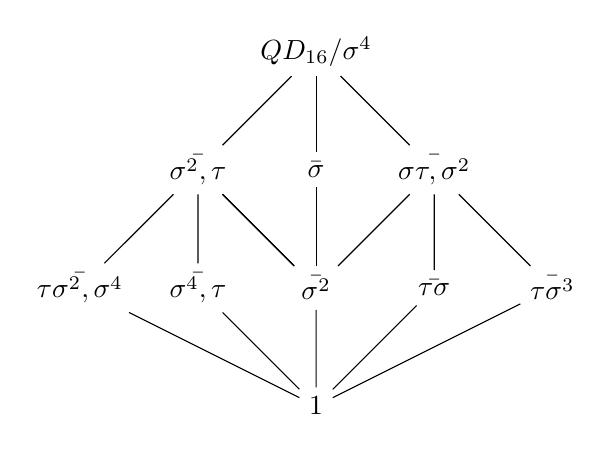
\begin{tikzpicture}[scale=1.5]
            \node (d8) at (0, 0) {$QD_{16}/\gen{\sigma^4}$};
            
            \node (sr2) at (-1, -1) {$\bar{\gen{\sigma^2, \tau}}$};
            \node (r) at (0, -1) {$\bar{\gen\sigma}$};
            \node (rsr2) at (1, -1) {${\bar{\gen{\sigma\tau, \sigma^2}}}$};

            \node (s) at (-2, -2) {$\bar{\gen{\tau\sigma^2, \sigma^4}}$};
            \node (r2s) at (-1, -2) {$\bar{\gen{\sigma^4, \tau}}$};
            \node (r2) at (0, -2) {$\bar{\gen{\sigma^2}}$};
            \node (rs) at (1, -2) {$\bar{\gen{\tau\sigma}}$};
            \node (r3s) at (2, -2) {$\bar{\gen{\tau\sigma^3}}$};
            
            \node (1) at (0, -3) {1};

            \draw (1) -- (s) -- (sr2) -- (d8);
            \draw (1) -- (r2s) -- (sr2);
            \draw (1) -- (r2) -- (sr2);
            \draw (1) -- (rs) -- (rsr2) -- (d8);
            \draw (1) -- (r3s) -- (rsr2);
            \draw (r2) -- (r) -- (d8);
            \draw (r2) -- (sr2);
            \draw (r2) -- (rsr2);
        \end{tikzpicture}
    \end{center}
    Moreover, $\bar{\sigma^4} = \bar{\tau^2} = \bar 1$ and $\bar{\tau\sigma} = \bar{\sigma^3\tau} = \bar{\sigma\inv\tau}$, then the generators $\bar\sigma$ and $\bar\tau$ satisfy the relations as $r$ and $s$ do in $D_8$, hence $QD_{16}/\gen{\sigma^4} \cong D_8$.
\end{sol}

\begin{exercise}
    Let $M = \gen{u, v}$ be the modular group of order 16 in \hyperref[ex2.5.14]{Exercise 2.5.14}. Prove that $\gen{v^4}$ is normal in $M$ and use the Lattice Isomorphism Theorem to draw the lattice of subgroups of $M/\gen{v^4}$. Which group of order 8 has the same lattice as this quotient? Use generators and relations for $M$ to decide the isomorphism type of this group.
\end{exercise}

\begin{sol}
    Note that $uv^4u = uuv^{20} = v^4$, hence $\gen{v^4} \nsub M$. By the Lattice Isomorphism Theorem, we may draw the following diagram:
    \begin{center}
        \begin{tikzpicture}[every node/.style=on grid]
            \node (G) {$M/\gen{v^4}$};

            \node (y) [below left=of G] {$\bar{\gen v}$};
            \node (xy) [below=of G] {$\bar{\gen{uv}}$};
            \node (x y2) [below right=of G] {$\bar{\gen{u, v^2}}$};

            \node (y2) [below right=of y] {$\bar{\gen{v^2}}$};
            \node (xy2) [below=of x y2] {$\bar{\gen{uv^2}}$};
            \node (x y4) [below right=of x y2] {$\bar{\gen{u, v^4}}$};

            \node (y4) [below right=of y2] {$\bar{\gen{v^4}}$};

            \draw (y4) -- (y2) -- (y) -- (G);
            \draw (y4) -- (x y4) -- (x y2) -- (G);
            \draw (y4) -- (xy2) -- (x y2);
            \draw (y2) -- (xy) -- (G);
            \draw (y2) -- (x y2);
        \end{tikzpicture}
    \end{center}
    Moreover, $\bar{v^4} = \bar{u^2} = \bar 1$ and $\bar{vu} = \bar{uv^5} = \bar{uv}$ so that the generators of $M/\gen{v^4}$ satisfy the relations as $a$ and $b$ do in $Z_2 \times Z_4$, whose presentation is given in \hyperref[ex2.5.12]{Exercise 2.5.12}. Then $M/\gen{v^4} \cong Z_2 \times Z_4$.
\end{sol}

\newpage

\begin{exercise}
    Let $M$ and $N$ be normal subgroups of $G$ such that $G = MN$. Prove that $G/(M \cap N) \cong (G/M) \times (G/N)$. [Draw the lattice.]
\end{exercise}

\begin{sol}
    The lattice is given as the following, where double lines represent the quotient group $G/(M \cap N)$:
    \begin{center}
        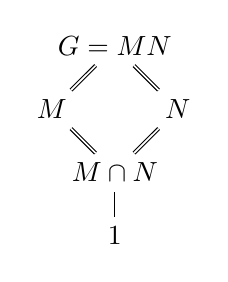
\begin{tikzpicture}[scale=0.8]
            \node (MN) at (0, 0) {$G = MN$};
            \node (M) at (-1, -1) {$M$};
            \node (N) at (1, -1) {$N$};
            \node (MnN) at (0, -2) {$M \cap N$};
            \node (1) at (0, -3) {1};

            \draw (1) -- (MnN);
            \draw [double] (MnN) -- (M) -- (MN);
            \draw [double] (MnN) -- (N) -- (MN);
        \end{tikzpicture}
    \end{center}
    Consider the mapping
    \[\phi : G \to (G/M) \times (G/N) \quad \text{by} \quad \phi(g) = (gM, gN)\]
    for $g \in G$. It is easy to see that $\phi$ is well-defined. Moreover, for any $g_1, g_2 \in G$,
    \[\phi(g_1g_2) = (g_1g_2M, g_1g_2N) = (g_1M, g_1N)(g_2M, g_2N) = \phi(g_1)\phi(g_2)\]
    so that $\phi$ is a homomorphism. To show that $\phi$ is surjective, let $(g_1M, g_2N) \in (G/M) \times (G/N)$ for some $g_1, g_2 \in G$. Since $G = MN = NM$, there exists $m, m' \in M$ and $n, n' \in N$ such that $g_1 = nm$ and $g_2 = m'n'$. Then $g_1M = nM$ and $g_2N = m'N$, so that
    \[\phi(nm') = (nm'M, nm'N) = (nM, m'N) = (g_1M, g_2N)\]
    so that $\phi$ is surjective. Lastly, suppose $g \in \ker\phi$. Then $\phi(g) = (M, N)$ so that $gM = M$ and $gN = N$. It follows that $g \in M$ and $g \in N$, hence $g \in M \cap N$. Therefore, $\ker\phi = M \cap N$, so that by the First Isomorphism Theorem, we have
    \[G/(M \cap N) \cong (G/M) \times (G/N). \qh\]
\end{sol}

\begin{exercise}
    Let $p$ be a prime and let $G$ be the group of $p$-power roots  of $1$ in $\c$ (cf. \hyperref[ex2.4.18]{Exercise 2.4.18}). Prove that the map $z \mapsto z^p$ is a surjective homomorphism. Deduce that $G$ is isomorphic to a proper quotient of itself.
\end{exercise}

\begin{sol}
    Let $\phi(z) = z^p$ be the map. For any $z, w \in G$, then $\phi(zw) = (zw)^p = z^p w^p = \phi(z)\phi(w)$, hence $\phi$ is a homomorphism. Moreover, for any $y \in G$, there is some $n \in \zp$ such that $y^{p^n} = 1$. Then let $z = y^{p^{n - 1}}$, so that $z^p = y^{p^n} = 1$, hence $z \in G$ and $\phi(z) = y$. It follows that $\phi$ is surjective. By the First Isomorphism Theorem, we have $G/\ker\phi \cong G$. Since $\ker\phi$ contains all $p$-power roots of unity of order dividing $p$, then $\ker\phi$ is nontrivial, hence $G$ is isomorphic to a proper quotient of itself.
\end{sol}

\begin{specialexercise}
    Let $p$ be a prime and let $G$ be a group of order $p^am$, where $p$ does not divide $m$. Assume $P$ is a subgroup of $G$ of order $p^a$ and $N$ is a normal subgroup of $G$ of order $p^b n$, where $p$ does not divide $n$. Prove that $|P \cap N| = p^b$ and $|PN/N| = p^{a - b}$. (The subgroup $P$ of $G$ is called a \textit{Sylow $p$-subgroup} of $G$. This exercise shows that the intersection of any Sylow $p$-subgroup with a normal subgroup $N$ is a Sylow $p$-subgroup of $N$.)
\end{specialexercise}

\begin{sol}
    Since $P \cap N \leq P$, then $|P \cap N|$ divides $|P| = p^a$. Similarly, since $P \cap N \leq N$, then $|P \cap N|$ divides $|N| = p^b n$. It follows that $|P \cap N|$ divides $\gcd(p^a, p^b n) = p^b$, hence $|P \cap N| = p^c$ for some $c \leq b$. By the Second Isomorphism Theorem, we have
    \[PN/N \cong P/(P \cap N)\]
    so that $|PN/N| = |P|/|P \cap N| = p^{a - c}$. Since $PN/N \leq G/N$, then $|PN/N|$ divides $|G/N|$. It follows that $p^{a - c}$ divides $|G|/|N| = (p^a m)/(p^b n) = p^{a - b}(m/n)$. Since $p$ does not divide $m/n$, then $p^{a - c}$ divides $p^{a - b}$, hence $c \geq b$. Therefore, $c = b$ so that $|P \cap N| = p^b$ and $|PN/N| = p^{a - b}$.
\end{sol}

\begin{exercise}
    Generalize the preceding exercise as follows. A subgroup $H$ of a finite group $G$ is called a \textit{Hall subgroup} of $G$ if its index in $G$ is relatively prime to its order: $(|G : H|, |H|) = 1$. Prove that if $H$ is a Hall subgroup of $G$ and $N \nsub G$, then $H \cap N$ is a Hall subgroup of $N$ and $HN/N$ is a Hall subgroup of $G/N$.
\end{exercise}

\begin{sol}
    It follows by the Second Isomorphism Theorem that $HN \leq G$ and $HN/N \cong H/(H \cap N)$. Note that
    \[|HN| = \frac{\abs H \abs N}{\abs{H \cap N}} \quad \text{must divide} \quad \abs G = \abs H |G : H|\]
    Hence, $|N|/\abs{H \cap N}$ divides $|G : H|$. Since $(|G : H|, \abs H) = 1$, and $|N|/|H \cap N|$ divides $|G : H|$, it follows that $(|N|/\abs{H \cap N}, \abs H) = 1$, hence $(\abs{N : H \cap N}, \abs{H \cap N}) = 1$. Then $H \cap N$ is a Hall subgroup of $N$.

    Now, observe that $|G/N : HN/N| = |G|/|HN| = |G:H|/|HN : H|$. Moreover, $|HN/N| = |H|/|H \cap N|$. Then $(|G/N : HN/N|, |HN/N|) = 1$ follows because $(|G : H|, \abs H) = 1$, hence $HN/N$ is a Hall subgroup of $G/N$.
\end{sol}

\newpage

\subsection{Composition Series and the H\"older Program}

\begin{exercise}
    Prove that if $G$ is an abelian simple group then $G \cong \mathbb{Z}_p$ for some prime $p$ (do not assume $G$ is a finite group).
\end{exercise}

\begin{sol}
    Since $G$ is abelian, every subgroup of $G$ is normal. Moreover, simplicity of $G$ implies that its only subgroups are 1 and $G$. If $G$ is the trivial group, then $G \cong Z_1$. Suppose $G$ is nontrivial, and let $g \in G$ be nonidentity. Then $\gen g \leq G$. Since $g \neq 1$ and $G$ is simple, then $\gen g = G$, hence $G$ is cyclic.

    Assume, by way of contradiction, that $\abs G$ is not prime. We have two cases:
    \begin{itemize}
        \item Suppose $\abs G$ is infinite. Then $G \cong \z$ has infinitely many proper nontrivial subgroups, contradicting the simplicity of $G$.
        \item Suppose $\abs G$ is finite and composite. Then there exists some divisor $d$ of $\abs G$ such that $1 < d < \abs G$. Since $G$ is cyclic, then there exists a unique subgroup of $G$ of order $d$, contradicting the simplicity of $G$.
    \end{itemize}
    Therefore, $\abs G$ is prime, and $G \cong Z_p$ for some prime $p$.
\end{sol}

\begin{exercise}
    Exhibit all $3$ composition series for $Q_8$ and all $7$ composition series for $D_8$. List the composition factors in each case.
\end{exercise}

\begin{sol}
    The composition series for $Q_8$ are as follows:
    \begin{align*}
        1 & \nsub \gen{-1} \nsub \gen i \nsub Q_8 \\
        1 & \nsub \gen{-1} \nsub \gen j \nsub Q_8 \\
        1 & \nsub \gen{-1} \nsub \gen k \nsub Q_8
    \end{align*}
    The composition factors for each series are isomorphic to $Z_2$.

    The composition series for $D_8$ are as follows:
    \begin{align*}
        1 & \nsub \gen s \nsub \gen{s, r^2} \nsub D_8 \\
        1 & \nsub \gen{r^2s} \nsub \gen{s, r^2} \nsub D_8 \\
        1 & \nsub \gen{r^2} \nsub \gen{s, r^2} \nsub D_8 \\
        1 & \nsub \gen{r^2} \nsub \gen r \nsub D_8 \\
        1 & \nsub \gen{r^2} \nsub \gen{rs, r^2} \nsub D_8 \\
        1 & \nsub \gen{rs} \nsub \gen{rs, r^2} \nsub D_8 \\
        1 & \nsub \gen{r^3s} \nsub \gen{rs, r^2} \nsub D_8
    \end{align*}
    with each composition factor isomorphic to $Z_2$.
\end{sol}

\begin{exercise}
    Find a composition series for the quasidihedral group of order $16$ (cf. \hyperref[ex2.5.11]{Exercise 2.5.11}). Deduce that $QD_{16}$ is solvable.
\end{exercise}

\begin{sol}
    A clear composition series is $1 \nsub \gen{\sigma^4} \nsub \gen{\sigma^2} \nsub \gen{\sigma} \nsub QD_{16}$, with each composition factor isomorphic to $Z_2$. Since all composition factors are abelian, then $QD_{16}$ is solvable.
\end{sol}

\newpage

\begin{exercise}
    Use Cauchy's Theorem and induction to show that a finite abelian group has a subgroup of order $n$ for each positive divisor $n$ of its order.
\end{exercise}

\begin{sol}
    Let $\abs G = m$. If $m = 1$, the result is trivial. We now proceed by induction on $m$.

    Suppose that every finite abelian group of order strictly less than $m$ has a subgroup of order $n$ for each positive divisor $n$ of its order. Let $n \in \zp$ where $n \mid m$. If $n$ is prime, then there exists $g \in G$ where $\abs g = n$ by Cauchy's Theorem. Then $\abs g \leq G$ is a subgroup of order $n$, and the result is true. 
    
    If $n$ is not prime, then $n = kp$ for some prime divisor $p$ of $n$. Since $p \mid m$, there exists an element $h \in G$ where $\abs h = p$ by Cauchy's Theorem. Then $\gen h$ has order $p$, and $G/\gen h$ is a finite abelian group of order $m/p < m$. Since $n$ divides $m$, then $k$ divides $m/p$. By the inductive hypothesis, there exists a subgroup $\bar H$ of $G/\gen h$ such that $\abs{\bar H} = k$. By the Lattice Isomorphism Theorem, there exists a subgroup $H$ of $G$ containing $\gen h$ such that $H/\gen h = \bar H$. Then $\abs H = \abs{\bar H} \abs{\gen h} = kp = n$, hence $H$ is a subgroup of $G$ of order $n$. By induction, the result holds for all finite abelian groups.
\end{sol}

\begin{specialexercise}
    Prove that subgroups and quotient groups of a solvable group are solvable.
\end{specialexercise}

\begin{sol}
    Let $G$ be a solveable group, and let $H \leq G$. Then there exists a chain of subgroups
    \[1 = G_0 \nsub G_1 \nsub \cdots \nsub G_n = G\]
    such that $G_{i + 1}/G_i$ is abelian. Define the subgroups
    \[H_i = H \cap G_i \quad \text{for each $0 \leq i \leq n$}\]
    Then $H_0 = H \cap G_0 = 1$ and $H_n = H \cap G_n = H$. It is clear that $H_i \leq H_{i + 1}$ for each $0 \leq i \leq n - 1$. To show that $H_i \nsub H_{i + 1}$, let $g \in H_{i + 1}$ and $x \in H_i$. Then $g \in G_{i + 1}$ and $x \in G_i$. Since $G_i \nsub G_{i + 1}$, then $gxg\inv \in G_i$. Since $g, x \in H$, then $gxg\inv \in H$, hence $gxg\inv \in H_i$. It follows that $H_i \nsub H_{i + 1}$. By the Second Isomorphism Theorem, we have
    \[H_{i + 1}/H_i \cong H_{i + 1}G_i/G_i \leq G_{i + 1}/G_i\]
    Since $G_{i + 1}/G_i$ is abelian, then so is $H_{i + 1}/H_i$. Therefore, $H$ is solvable with the chain
    \[1 = H_0 \nsub H_1 \nsub \cdots \nsub H_n = H\]
    Now let $N \nsub G$. Consider the subgroups
    \[N_i = G_iN \quad \text{for each $0 \leq i \leq n$}\]
    Since it is clear that $N_i \leq N_{i + 1}$, we need to show that $N_i \nsub N_{i + 1}$. Let $g \in G_{i + 1}, h \in G_i$, and $n_1, n_2 \in N$. Then
    \[(gn_1)(hn_2)(gn_1)\inv = g n_1 h n_2 n_1\inv g\inv = g(n_1 h n_2 n_1\inv)g \inv\]
    Note that $n_1 hn_2n_1\inv \in N_i$ since $h \in G_i \leq G$ and $N \nsub G$. Since $G_i \nsub G_{i + 1}$, then $g(n_1 h n_2 n_1\inv)g \inv \in G_i \subseteq N_i$. It follows that $N_i \nsub N_{i + 1}$.

    Lastly, by the Lattice Isomorphism Theorem, then $N_i/N \nsub N_{i + 1}/N$, and the Third Isomorphism Theorem concludes that
    \[(N_{i + 1}/N)/(N_i/N) \cong N_{i + 1}/N_i \cong G_{i + 1}/(G_iN \cap G_{i + 1}) = G_{i + 1}/G_i\]
    Since $G_{i + 1}/G_i$ is abelian, then so is $(N_{i + 1}/N)/(N_i/N)$. Therefore, $G/N$ is solvable with the chain
    \[1 = N_0/N \nsub N_1/N \nsub \cdots \nsub N_n/N = G/N. \qh\]
\end{sol}

\newpage

\begin{exercise}
    Prove part (1) of the Jordan--H\"older Theorem by induction on $|G|$.
\end{exercise}

\begin{sol}
    Let $G$ be a finite group. If $G = 1$, then the result is trivial. Suppose now $G$ is nontrivial and that the result holds for all groups of order less than $\abs G$. If $G$ is simple, then the composition series is $1 \nsub G$. Suppose now $G$ is not simple, and let $N$ be a maximal, normal subgroup of $G$. Since $\abs N < \abs G$, we may conclude by the inductive hypothesis that there exists a composition series
    \[1 = N_0 \nsub N_1 \nsub \cdots \nsub N_k = N\]
    for some $k \in \zp$. Since $N \nsub G$ and $G/N$ is simple, then the chain
    \[1 = N_0 \nsub N_1 \nsub \cdots \nsub N_k = N \nsub G\]
    is a composition series for $G$. By induction, the result holds for all finite groups.
\end{sol}

\begin{exercise}
    If $G$ is a finite group and $H \trianglelefteq G$, prove that there is a composition series of $G$, one of whose terms is $H$.
\end{exercise}

\begin{sol}
    If $H = G$, then the result follows trivially, since the last term in the composition series must be $H$. Now suppose $H$ is a proper, normal subgroup of $G$. If $\abs G = 1$, the result is trivial. Suppose $\abs G > 1$, and assume the result is true for all groups with order less than $\abs G$.

    Since $H$ is proper, then $\abs H < \abs G$, hence we have a composition series
    \[1 = H_0 \nsub H_1 \nsub \cdots \nsub H_m = H\]
    by the inductive hypothesis. Now consider the quotient group $G/H$. Since $\abs{G/H} < \abs G$, then by the inductive hypothesis, there exists a composition series
    \[1 = K_0/H \nsub K_1/H \nsub \cdots \nsub K_n/H = G/H\]
    for some $n \in \zp$. By the Lattice Isomorphism Theorem, we have $H = K_0 \nsub K_1 \nsub \cdots \nsub K_n = G$. Since each $K_{i + 1}/K_i \cong (K_{i + 1}/H)/(K_i/H)$ is simple, then the chain
    \[1 = H_0 \nsub H_1 \nsub \cdots \nsub H_m = H = K_0 \nsub K_1 \nsub \cdots \nsub K_n = G\]
    is a composition series for $G$ with one of its terms equal to $H$. By induction, the result holds for all finite groups.
\end{sol}

\begin{exercise}
    Let $G$ be a \textit{finite} group. Prove that the following are equivalent:
    \begin{enumerate}
        \item[(i)] $G$ is solvable.
        \item[(ii)] $G$ has a chain of subgroups
        \[1 = H_0 \trianglelefteq H_1 \trianglelefteq H_2 \trianglelefteq \cdots \trianglelefteq H_s = G\]
        such that $H_{i+1}/H_i$ is cyclic, $0 \le i \le s-1$.
        \item[(iii)] All composition factors of $G$ are of prime order.
        \item[(iv)] $G$ has a chain of subgroups
        \[1 = N_0 \trianglelefteq N_1 \trianglelefteq N_2 \trianglelefteq \cdots \trianglelefteq N_t = G\]
        such that each $N_i$ is a normal subgroup of $G$ and $N_{i+1}/N_i$ is abelian, $0 \le i \le t-1$.
    \end{enumerate}
    \noindent [For (iv), prove that a minimal nontrivial normal subgroup $M$ of $G$ is necessarily abelian and then use induction. To see that $M$ is abelian, let $N \trianglelefteq M$ be of prime index (by (iii)) and show that $x^{-1}y^{-1}xy \in N$ for all $x,y \in M$ (cf. \hyperref[ex3.1.40]{Exercise 3.1.40}). Apply the same argument to $gNg^{-1}$ to show that $x^{-1}y^{-1}xy$ lies in the intersection of all $G$-conjugates of $N$, and use the minimality of $M$ to conclude that $x^{-1}y^{-1}xy = 1$.]
\end{exercise}

\begin{sol}
    \textbf{(i) \rightimp (ii)}: Suppose $G$ is solvable, and consider the chain of subgroups
    \[1 = G_0 \nsub G_1 \nsub \cdots \nsub G_n = G\]
    where $G_{i + 1}/G_i$ is abelian. We prove the following lemma: if $A$ is a finite abelian group, then there exists a chain of subgroups
    \[1 = A_0 \nsub A_1 \nsub \cdots \nsub A_k = A\]
    such that $A_{j + 1}/A_j$ is cyclic. We prove this lemma by induction on $\abs A$. If $\abs A = 1$, the result is trivial. Suppose $\abs A > 1$ and that the result holds for all abelian groups of order less than $\abs A$. Since $A$ is finite abelian, there exists some nonidentity $a \in A$ such that $\gen a \nsub A$. Then $\abs{\gen a} < \abs A$, hence by the inductive hypothesis, there exists a chain of subgroups
    \[1 = B_0 \nsub B_1 \nsub \cdots \nsub B_m = \gen a\]
    such that $B_{j + 1}/B_j$ is cyclic. Now consider the quotient group $A/\gen a$. Since $\abs{A/\gen a} < \abs A$, then by the inductive hypothesis, there exists a chain of subgroups
    \[1 = C_0/\gen a \nsub C_1/\gen a \nsub \cdots \nsub C_\ell/\gen a = A/\gen a\]
    for some $\ell \in \zp$. By the Lattice Isomorphism Theorem, we have $\gen a = C_0 \nsub C_1 \nsub \cdots \nsub C_\ell = A$. Since each $C_{i + 1}/C_i \cong (C_{i + 1}/\gen a)/(C_i/\gen a)$ is cyclic, then the chain
    \[1 = B_0 \nsub B_1 \nsub \cdots \nsub B_m = \gen a = C_0 \nsub C_1 \nsub \cdots \nsub C_\ell = A\]
    satisfies the lemma. By induction, the lemma holds for all finite abelian groups. 

    Applying this lemma to each abelian quotient $G_{i + 1}/G_i$ in the original chain, we obtain a chain of subgroups
    \[1 = H_0 \nsub H_1 \nsub H_2 \nsub \cdots \nsub H_s = G\]
    such that $H_{i + 1}/H_i$ is cyclic, hence (ii) holds.

    \textbf{(ii) \rightimp (iii)}: Suppose $G$ has a chain of subgroups
    \[1 = H_0 \nsub H_1 \nsub H_2 \nsub \cdots \nsub H_s = G\]
    such that $H_{i + 1}/H_i$ is cyclic. We prove that each composition factor of $G$ is of prime order. We prove this by induction on $\abs G$. If $\abs G = 1$, the result is trivial. Suppose $\abs G > 1$ and that the result holds for all groups of order less than $\abs G$. Since $H_{s - 1} \nsub G$ and $G/H_{s - 1}$ is cyclic, then $G/H_{s - 1} \cong Z_n$ for some $n \in \zp$. If $n$ is prime, then the composition factors of $G/H_{s - 1}$ are of prime order. Since $\abs{H_{s - 1}} < \abs G$, then by the inductive hypothesis, the composition factors of $H_{s - 1}$ are also of prime order, hence all composition factors of $G$ are of prime order. Suppose now $n$ is not prime, so that $n = km$ for some $k, m \in \zp$ where $1 < k, m < n$. Then $Z_n$ has a proper, nontrivial subgroup $\gen{a^m}$ of order $k$. Let $\pi : G \to G/H_{s - 1}$ be the natural projection, and let $K = \pi\inv(\gen{a^m})$. Then $H_{s - 1} \nsub K \nsub G$ so that by the Lattice Isomorphism Theorem, $K/H_{s - 1} \cong \gen{a^m}$ is a proper, nontrivial subgroup of $G/H_{s - 1}$, contradicting that $H_{s - 1}$ is maximal normal in $G$. It follows that $n$ must be prime, hence all composition factors of $G$ are of prime order. By induction, the result holds for all finite groups.

    \textbf{(iii) \rightimp (iv)}: Suppose all composition factors of $G$ are of prime order. We prove that $G$ has a chain of subgroups
    \[1 = N_0 \nsub N_1 \nsub N_2 \nsub \cdots \nsub N_t = G\]
    such that each $N_i$ is a normal subgroup of $G$ and $N_{i + 1}/N_i$ is abelian. Let $M$ be a minimal, nontrivial normal subgroup of $G$, and suppose $N \nsub M$ have prime index. Then for any $x, y \in M$, we have $x^{-1}y^{-1}xy \in N$ since $M/N$ is abelian. Now for any $g \in G$, consider $gNg\inv \nsub gMg\inv = M$. By the same argument, we have $x^{-1}y^{-1}xy \in gNg\inv$ for all $x, y \in M$. It follows that $x^{-1}y^{-1}xy$ lies in the intersection of all $G$-conjugates of $N$. Since $M$ is minimal normal in $G$, then this intersection is either 1 or $M$. If it were $M$, then $M$ would be abelian, contradicting that $M/N$ is nontrivial. Hence, $x^{-1}y^{-1}xy = 1$ for all $x, y \in M$, so that $M$ is abelian.

    \textbf{(iv) \rightimp (i)}: This implication is immediate from the definition of solvable groups.
\end{sol}

\begin{exercise}
    Prove the following special case of part (2) of the Jordan--H\"older Theorem: assume the finite group $G$ has two composition series
    \[ 1 = N_0 \trianglelefteq N_1 \trianglelefteq \cdots \trianglelefteq N_r = G \quad\text{and}\quad 1 = M_0 \trianglelefteq M_1 \trianglelefteq M_2 = G. \]
    Show that $r = 2$ and that the list of composition factors is the same. [Use the Second Isomorphism Theorem.]
\end{exercise}

\begin{sol}
    Consider $H = N_{r - 1} \cap M_1$. Then $H \nsub M_1$. Since $M_1/1 \cong M_1$ is simple, then either $H = 1$ or $H = M_1$. If $H = M_1$, then $N_{r - 1} \nsub M_1$. By simplicity of $M_1$, it must be that $N_{r - 1} = M_1$ so that $r = 2$. Both composition series are then the same, so we now suppose $H = 1$.

    Noting that $M_1 \nsub G$ and $N_{r - 1} \nsub G$, we may use the Second Isomorphism Theorem to conclude that
    \[N_{r - 1}M_1/M_1 \cong N_{r - 1}/(N_{r - 1} \cap M_1) = N_{r - 1}/1 \cong N_{r - 1}.\] Observe now that $M_1 \leq N_{r - 1}M_1 \leq G$, hence $N_{r - 1}M_1/M_1 \nsub G/M_1$. By simplicity of $G/M_1$, it must be that $N_{r - 1}M_1 = 1$ or $N_{r - 1}M_1 = G$. Since $N_{r - 1}$ is not trivial, it must be that $N_{r - 1}M_1 = G$. Now, $N_{r - 1}$ is simple, hence $N_{r - 2} = 1 = N_0$, and we may conclude that $r = 2$. Moreover, the composition factors are isomorphic:
    \[G/N_{r - 1} \cong M_1/(N_{r - 1} \cap M_1) \cong M_1 \quad \text{and} \quad N_{r - 1}/1 \cong N_{r - 1} \cong G/M_1 \qh\]
\end{sol}

\begin{exercise}
    Prove part (2) of the Jordan--H\"older Theorem by induction on $\min\{r,s\}$. [Apply the inductive hypothesis to $H = N_{r-1} \cap M_{s-1}$ and use the preceding exercises.]
\end{exercise}

\begin{sol}
    Suppose $G$ has two composition series
    \begin{equation}
        \label{eqclubsuit}
        \tag{$\clubsuit$}
        1 = N_0 \nsub N_1 \nsub \cdots \nsub N_r = G
    \end{equation}
    and
    \begin{equation}
        \label{eqspadesuit}
        \tag{$\spadesuit$}
        1 = M_0 \nsub M_1 \nsub \cdots \nsub M_s = G.
    \end{equation}
    We induct on $\min\set{r,s}$. By the previous exercise, we may assume that $\min\set{r, s} > 2$. Suppose the statement is true for $\min\set{r, s} < k$ for some $k > 2$, and let $\min\set{r, s} = k$. Let $H = N_{r - 1} \cap M_{s - 1}$. If $N_{r - 1} \leq M_{s - 1}$ is proper, then by simplicity of $M_{s - 1}$, it must be that $N_{r - 1} = 1$, contradicting that $N_{r - 1}$ is nontrivial. Hence, $N_{r - 1} \nsub M_{s - 1}$. By a similar argument, we have $M_{s - 1} \nsub N_{r - 1}$. If we have $M_{s - 1} = N_{r - 1}$, then by the previous exercise, the composition factors of both series are the same, so we now suppose $M_{s - 1} \neq N_{r - 1}$ and they are not contained 
    in one another. They are then proper normal subgroups of $M_{s - 1}N_{r - 1}$. If $M_{s - 1}N_{r - 1} \neq G$, then $M_{s - 1}N_{r - 1} \nsub G$ is proper, so by simplicity of $G/N_{r - 1}$, it must be that $M_{s - 1}N_{r - 1} = N_{r - 1}$, contradicting that $M_{s - 1} \nsub N_{r - 1}$. Hence, $M_{s - 1}N_{r - 1} = G$. We may use the Second Isomorphism Theorem to conclude that
    \begin{equation}
        \label{eqheartsuit}
        \tag{$\heartsuit$}
        M_{s - 1}/H \cong M_{s - 1}N_{r - 1}/N_{r - 1} = G/N_{r - 1}
    \end{equation}
    and
    \begin{equation}
        \label{eqdiamondsuit}
        \tag{$\diamondsuit$}
        N_{r - 1}/H \cong M_{s - 1}N_{r - 1}/M_{s - 1} = G/M_{s - 1}.
    \end{equation}
    which shows that both $M_{s - 1}/H$ and $N_{r - 1}/H$ are simple. Consider now the composition series for $H$:
    \begin{equation}
        \label{eqstar}
        \tag{$\star$}
        1 = H_0 \nsub H_1 \nsub \cdots \nsub H_t = H.
    \end{equation}
    It is clear that appending $N_{r - 1}$ to the series \eqref{eqstar} gives a composition series for $N_{r - 1}$. Similarly, we get a composition series for $M_{s - 1}$. Moreover, there are $r - 2$ factors for the series for $N_{r - 1}$ and $s - 2$ factors for the series for $M_{s - 1}$. Since $\min\set{r - 1, s - 1} = k - 1 < k$, then by the inductive hypothesis, both series have the same number of factors and the same composition factors up to isomorphism. Therefore, $r - 2 = s - 2$ so that $r = s$. In \eqref{eqclubsuit} and \eqref{eqspadesuit}, both series have $r - 2$ factors isomorphic to \eqref{eqstar} up to some order, and the last 2 factors in \eqref{eqheartsuit} and \eqref{eqdiamondsuit} are isomorphic to $G/N_{r - 1}$ and $G/M_{s - 1}$ respectively. The result then follows by induction.
\end{sol}

\begin{exercise}
    Prove that if $H$ is a nontrivial normal subgroup of the solvable group $G$ then there is a nontrivial subgroup $A$ of $H$ with $A \trianglelefteq G$ and $A$ abelian.
\end{exercise}

\begin{sol}
    Since $G$ is solvable, we have the sequence
    \[1 = G_0 \nsub G_1 \nsub \cdots \nsub G_n = G\]
    where $G_{i + 1}/G_i$ is abelian. Let $H_i = H \cap G_i$ for each $0 \leq i \leq n$. Since $H$ is nontrivial, consider the set of indices $I = \set{i \in \zp \mid G_i \cap H \neq 1}$. Since $H_n = H$, then $I$ is nonempty. By the Well Ordering Property, there exist some minimal index $k$ such that $H_k = G_k \cap H \neq 1$ but $H_{k - 1} = G_{k - 1} \cap H = 1$. Note that $H_k \nsub G$ since $H \nsub G$ and $G_k \nsub G$. Moreover, by the Second Isomorphism Theorem, we have
    \[H_k \cong H_k/1 = H_k/(H_k \cap G_{k - 1}) \cong H_k G_{k - 1}/G_{k - 1} \leq G_k/G_{k - 1}\]
    Since $G_k/G_{k - 1}$ is abelian, then so is $H_k$. Therefore, $A = H_k$ is a nontrivial, abelian normal subgroup of $G$ contained in $H$.
\end{sol}

\begin{exercise}
    Prove (without using the Feit--Thompson Theorem) that the following are equivalent:
    \begin{enumerate}
    \item[(i)] Every group of odd order is solvable.
    \item[(ii)] The only simple groups of odd order are those of prime order.
    \end{enumerate}
\end{exercise}

\begin{sol}
    \textbf{(i) \rightimp (ii)} Suppose every group of odd order is solvable. Let $G$ be a simple group of odd order. Since $G$ is solvable, then by the characterization of solvable groups, all composition factors of $G$ are of prime order. Since $G$ is simple, then its only composition series is $1 \nsub G$, hence $G$ is of prime order.

    \noindent \textbf{(ii) \rightimp (i)} Suppose the only simple groups of odd order are those of prime order. Let $G$ be a group of odd order. We want to show that $G$ is solvable. Consider a composition series of $G$:
    \[1 = G_0 \nsub G_1 \nsub \cdots \nsub G_n = G.\]
    Each composition factor $G_{i+1}/G_i$ is simple and of odd order, so by assumption, each is of prime order and hence abelian. Therefore, $G$ is solvable.
\end{sol}

\newpage

\subsection{Transpositions and the Alternating Group}

\begin{exercise}
    In \hyperref[ex1.3.1]{Exercise 1.3.1} and \hyperref[ex1.3.2]{Exercise 1.3.2} you were asked to find the cycle decomposition of some permutations. Write each of these permutations as a product of transpositions. Determine which of these is an even permutation and which is an odd permutation.
\end{exercise}

\begin{sol}
    For \hyperref[ex1.3.1]{Exercise 1.3.1}, odd permutations are $\sigma$, $\sigma\tau$, $\tau\sigma$, and $\tau^2\sigma$, while even permutations are $\tau$ and $\sigma^2$. For \hyperref[ex1.3.2]{Exercise 1.3.2}, odd permutations are $\tau$, $\tau\sigma$, and $\tau^2\sigma$, while even permutations are $\sigma, \sigma^2$, and $\sigma\tau$.
\end{sol}

\begin{exercise}
    Prove that $\sigma^2$ is an even permutation for every permutation $\sigma$.
\end{exercise}

\begin{sol}
    Let $\sigma$ be a permutation with a transposition product $\tau_1\tau_2 \cdots \tau_k$. Then $\sigma^2$ has $2k$ transpositions in its product, hence is even.
\end{sol}

\begin{exercise}
    Prove that $S_n$ is generated by $\{(i\ i+1)\mid 1 \le i \le n-1\}$. [Consider conjugates, viz.\ $(2\ 3)(1\ 2)(2\ 3)^{-1}$.]
\end{exercise}

\begin{sol}
    Inducting on $n$, note that the base case is trivial. Let $T_n = \gen{(i\ i + 1) \mid 1 \leq i \leq n - 1}$. Suppose that $S_n = T_n$ for some $n \geq 1$, and consider some $\sigma \in S_{n + 1}$. Write $\sigma$ as a product of transpositions, and let $(j\ k)$ be a transposition in $\sigma$.

    There are 2 cases to consider. If $1 \leq j < k \leq n$, then $(j\ k) \in S_n = T_n$ by the inductive hypothesis. If $k = n + 1$ and $j = n$, then $(j\ k) \in T_{n + 1}$ by definition. Suppose now that $1 \leq j < k = n + 1$ where $j < n$. Note that
    \[(j\ n + 1) = (n\ n + 1)(j\ n)(n\ n + 1)\]
    where each transposition on the right-hand side is in $T_{n + 1}$ (in particular, $(j\ n) \in S_n = T_n$ by the inductive hypothesis). It follows that $(j\ k) \in T_{n + 1}$ for all transpositions in $\sigma$, hence $\sigma \in T_{n + 1}$. By induction, the result holds for all $n \geq 1$.
\end{sol}

\begin{exercise}
    Show that $S_n=\langle (1\ 2),(1\ 2\ 3 \ldots n)\rangle$ for all $n\ge2$.
\end{exercise}

\begin{sol}
    Note that $(1\ 2\ 3 \ldots n)(1\ 2)(1\ 2\ 3 \ldots n)^{-1} = (2\ 3)$. We may conjugate $(2\ 3)$ by the $n$-cycle again to get $(3\ 4)$, and so on until an arbitrary $(i\ i + 1) = (1\ 2\ 3 \ldots n)^{i - 1}(1\ 2)(1\ 2\ 3 \ldots n)^{-(i - 1)}$ is obtained for each $1 \leq i < n$. By the previous exercise, then $S_n = \gen{(1\ 2), (1\ 2\ 3 \ldots n)}$.
\end{sol}

\begin{exercise}
    Show that if $p$ is prime, $S_p=\langle \sigma,\tau\rangle$ where $\sigma$ is any transposition and $\tau$ is any $p$-cycle.
\end{exercise}

\begin{sol}
    It is clear that the set of all transpositions is equal to $S_n$, since any permutation in $S_n$ can be written as a product of transpositions. Let $\sigma = (i\ j)$ and $\tau$ be a $p$-cycle. Note that there exists some power $k$ such that $\tau^k(i) = 1$. Then $\sigma' = \tau^k\sigma\tau^{-k} = (1\ \tau^k(j))$ is a transposition in $\gen{\sigma, \tau}$. We claim that every transposition of the form $(1\ k) \in \gen{\sigma, \tau}$ for $2 \leq k \leq p$, and we proceed by induction. The base case of $(1\ \tau^k(j))$ is done. Suppose $(1\ m) \in \gen{\sigma, \tau}$ for some $2 \leq m < p$. Note that there must exist some power $n$ such that $\tau^n(1) = m$. Then $\tau^n(1\ \tau^k(j))\tau^{-n} = (m\ \tau^{n + k}(j))$ lies in $\gen{\sigma, \tau}$. Then $(1\ \tau^{n + k}(j)) = (1\ m)(m\ \tau^{n + k}(j))(1\ m) \in \gen{\sigma, \tau}$. By induction, every transposition of the form $(1\ k)$ is in $\gen{\sigma, \tau}$. Then for any transposition $(a\ b)$, we have $(a\ b) = (1\ a)(1\ b)(1\ a) \in \gen{\sigma, \tau}$. It follows that all transpositions are in $\gen{\sigma, \tau}$, hence $S_p = \gen{\sigma, \tau}$.
\end{sol}

\begin{exercise}
    Show that $\langle (1\ 3),(1\ 2\ 3\ 4)\rangle$ is a proper subgroup of $S_4$. What is the isomorphism type of this subgroup?
\end{exercise}

\begin{sol}
    Put $\tau = (1\ 3)$ and $\sigma = (1\ 2\ 3\ 4)$. Then $\sigma^4 = \tau^2 = 1$. Moreover, $\sigma\tau = (1\ 2\ 3\ 4)(1\ 3) = (1\ 4)(2\ 3)$, and $\tau\sigma\inv = (1\ 3)(4\ 3\ 2\ 1) = (1\ 4)(2\ 3)$, so that $\sigma\tau = \tau\sigma\inv$. This satisfies the same relations in $S_4$ as $r$ and $s$ do in $D_8$. We then define a surjective homomorphism $\phi : D_8 \to \gen{\sigma, \tau}$ by $\phi(r) = \sigma$ and $\phi(s) = \tau$. Then $\gen{\sigma, \tau}$ has at most 8 elements, showing that it is a proper subgroup of $S_4$. It is easy to see that $\phi$ maps to distinct elements in $\gen{\sigma, \tau}$, hence $\abs{\gen{\sigma, \tau}} = 8$ and $\phi$ is an isomorphism. Therefore, $\gen{\sigma, \tau} \cong D_8$.
\end{sol}

\begin{exercise}
    Prove that the group of rigid motions of a tetrahedron is isomorphic to $A_4$. [Recall \hyperref[ex1.7.20]{Exercise 1.7.20}.]
\end{exercise}

\begin{sol}
    By \hyperref[ex1.7.20]{Exercise 1.7.20}, we know that the group of rigid motions is isomorphic to a subgroup of $S_4$. Moreover, \hyperref[ex1.2.9]{Exercise 1.2.9} shows that this group has order 12. We claim that the subgroup of $S_4$ that this group is isomorphic to is $A_4$. 

    The group of rigid motions of a tetrahedron consists of the following elements: the identity, 8 rotations about axes through a vertex and the center of the opposite face (by $120^\circ$ or $240^\circ$), and 3 rotations about axes through the midpoints of opposite edges (by $180^\circ$). The identity is even, the 8 rotations about vertices are even (since they correspond to $3$-cycles in $S_4$), and the 3 rotations about midpoints of edges are also even (since they correspond to products of two disjoint transpositions in $S_4$). Therefore, all 12 elements of the group of rigid motions are even permutations, so the group is isomorphic to a subgroup of $A_4$. Since both groups have order 12, it follows that the group of rigid motions of a tetrahedron is isomorphic to $A_4$.
\end{sol}

\begin{exercise}
    \label{ex3.5.8} Prove the lattice of subgroups of $A_4$ given in the text is correct. (By the preceding exercise and the comments following Lagrange's Theorem, $A_4$ has no subgroup of order $6$.)
\end{exercise}

\begin{sol}
    The previous exercise shows that $A_4$ is isomorphic to the group of rigid motions of a tetrahedron, where the text shows that this group cannot have a subgroup of order 6.

    We know that a subgroup of $A_4$ with order 4 must be isomorphic to either $Z_4$ or $V_4$. Since the symmetries of $A_4$ have either order 1 (the identity), order 2 (the $180^\circ$ rotations about midpoints of opposite edges), or order 3 (the $120^\circ$ and $240^\circ$ rotations about vertices), there are no elements of order 4 in $A_4$. Therefore, the unique subgroup of order 4 in $A_4$ must be isomorphic to $V_4$, namely $\gen{(1\ 2)(3\ 4), (1\ 3)(2\ 4)}$. Moreover, this is the only subgroup of order 4 in $A_4$ since any other subgroup of order 4 would necessarily contain different elements of order 2, which there are none of besides in this subgroup.

    The remaining potential subgroup orders of $A_4$ are 2 or 3, both of which are cyclic. Since the lattice shows 4 cyclic subgroups of order 3 that contain all 8 elements of order 3 in $A_4$, and 3 cyclic subgroups of order 2 that contain all 3 elements of order 2 in $A_4$, the lattice is correct.
\end{sol}

\begin{exercise}
    \label{ex3.5.9} Prove that the (unique) subgroup of order $4$ in $A_4$ is normal and is isomorphic to $V_4$.
\end{exercise}

\begin{sol}
    The above discussion shows that $A_4$ is isomorphic to $V_4$. Moreover, this subgroup is generated by all elements of order 2 in $A_4$. By \hyperref[ex3.1.26]{Exercise 3.1.26}, this subgroup is normal in $A_4$.
\end{sol}

\newpage

\begin{exercise}
    Find a composition series for $A_4$. Deduce that $A_4$ is solvable.
\end{exercise}

\begin{sol}
    Since the subgroup lattice is correct, we know that the subgroup of order 4 is maximal and normal in $A_4$. Moreover, it is abelian. Therefore, we have the composition series
    \[1 \nsub \gen{(1\ 2)(3\ 4)} \nsub \gen{(1\ 2)(3\ 4), (1\ 3)(2\ 4)} \nsub A_4\]
    where each composition factor is of prime order. By the characterization of solvable groups, $A_4$ is solvable.
\end{sol}

\begin{exercise}
    Prove that $S_4$ has no subgroup isomorphic to $Q_8$.
\end{exercise}

\begin{sol}
    If such a subgroup $H$ of $S_4$ existed, then it would contain all elements of order 4 in $S_4$ (of which there are 6) since $Q_8$ has 6 elements of order 4. However, this implies that $(1\ 2\ 3\ 4)^2 = (1\ 3)(2\ 4) \in H$ and $(1\ 4\ 3\ 2)^2 = (1\ 4)(2\ 3) \in H$. Along with the identity, this shows that $H$ contains more than 8 elements, a contradiction. Therefore, no such subgroup exists.
\end{sol}

\begin{exercise}
    Prove that $A_n$ contains a subgroup isomorphic to $S_{n-2}$ for each $n\ge3$.
\end{exercise}

\begin{sol}
    Recall that $A_n$ contains only even permutations, while $S_{n - 2}$ contain both even and odd permutations. Our homomorphism must then mapp odd permutations of $S_{n - 2}$ to even permutations of $A_n$, while ensuring that the original action of the permutation in $S_{n - 2}$ is preserved. Hence, we ``add'' on a transposition to odd permutations in $S_{n - 2}$ to make them even in $A_n$. We then define the map $\phi: S_{n - 2} \to A_n$ by
    \[\phi(\sigma) = 
    \begin{cases}
        \sigma & \text{if $\sigma$ is even,}\\
        \sigma \circ (n - 1\ n) & \text{if $\sigma$ is odd.}
    \end{cases}\]
    Now suppose $\sigma, \tau \in S_{n - 2}$. There are 3 cases to consider:
    \begin{enumerate}
        \item If both $\sigma$ and $\tau$ are even, then $\phi(\sigma\tau) = \sigma\tau = \phi(\sigma)\phi(\tau)$.
        \item If both $\sigma$ and $\tau$ are odd, then $\phi(\sigma\tau) = \sigma \circ (n - 1\ n)\tau \circ (n - 1\ n) = \phi(\sigma)\phi(\tau)$.
        \item Without loss of generality, assume $\sigma$ is even and $\tau$ is odd. Then $\phi(\sigma\tau) = \sigma\tau \circ (n - 1\ n) = \phi(\sigma)\phi(\tau)$.
    \end{enumerate}
    In all cases, $\phi(\sigma\tau) = \phi(\sigma)\phi(\tau)$, so $\phi$ is a homomorphism. It is clear that $\phi$ is injective, since if $\phi(\sigma) = \phi(\tau)$, then either both $\sigma$ and $\tau$ are even or both are odd, so that $\sigma = \tau$. Therefore, $\phi$ is an injective homomorphism from $S_{n - 2}$ to $A_n$, showing that $A_n$ contains a subgroup isomorphic to $S_{n - 2}$.
\end{sol}

\begin{exercise}
    Prove that every element of order $2$ in $A_n$ is the square of an element of order $4$ in $S_n$. [An element of order $2$ in $A_n$ is a product of $2k$ commuting transpositions.]
\end{exercise}

\begin{sol}
    By the hint, every element of order 2 in $A_n$ contains a pair of cycles of the form $(a\ b)(c\ d)$. Note that $(a\ c\ b\ d)^2 = (a\ b)(c\ d)$, and $(a\ c\ b\ d)$ is of order 4 in $S_n$. Then any element of order 2 in $A_n$ can be written as the square of an element of order 4 in $S_n$ by grouping its transpositions into pairs and applying this construction to each pair.
\end{sol}

\begin{exercise}
    Prove that the subgroup of $A_4$ generated by any element of order $2$ and any element of order $3$ is all of $A_4$.
\end{exercise}

\begin{sol}
    Observing the lattice was proven correct in \hyperref[ex3.5.8]{Exercise 3.5.8}, we see that any subgroup generated by an element $\sigma$ of order 2 and an element $\tau$ of order 3. Then $\gen{\sigma}$ is a proper subgroup of $\gen{\sigma, \tau}$, but the lattice shows that $\gen{\sigma}$ is maximal in $A_4$. Therefore, $\gen{\sigma, \tau} = A_4$.
\end{sol}

\begin{exercise}
    Prove that if $x$ and $y$ are distinct $3$-cycles in $S_4$ with $x \ne y^{-1}$, then the subgroup of $S_4$ generated by $x$ and $y$ is $A_4$.
\end{exercise}

\begin{sol}
    Using the same argument in the previous exercise, we note that $\gen x$ and $\gen y$ are distinct, proper subgroups of $\gen{x, y}$. Since both are maximal in $A_4$, it follows that $\gen{x, y} = A_4$.
\end{sol}

\begin{exercise}
    Let $x$ and $y$ be distinct $3$-cycles in $S_5$ with $x\ne y^{-1}$.
    \begin{subproblems}
    \item Prove that if $x$ and $y$ fix a common element of $\{1,\dots,5\}$, then $\langle x,y\rangle \cong A_4$.
    \item Prove that if $x$ and $y$ do not fix a common element of $\{1,\dots,5\}$, then $\langle x,y\rangle = A_5$.
    \end{subproblems}
\end{exercise}

\begin{solalph}
    \item Consider $X = \set{1, 2, 3, 4, 5} - \set i$, where $i \in \set{1, 2, 3, 4, 5}$ is the common element being fixed by both $x$ and $y$. Then $x$ and $y$ act only on $X$. Define the map $\phi : \gen{x, y} \to S_4$ given by $\phi(\sigma) = \sigma|_X$. It is clear that $\phi$ is a homomorphism. 
    
    Now suppose $\sigma \in \ker\phi$. Then $\sigma$ fixes all elements in $X$ as well as $i$, so that $\sigma$ is the identity. Therefore, $\phi$ is injective. We now look at $\phi(\gen{x, y}) = \gen{\phi(x), \phi(y)}$. Since $\phi$ is injective, it follows that $\phi(x) \neq \phi(y)$ and $\phi(x) \neq \phi(y)\inv$ if $x \neq y$ and $x \neq y\inv$. By the previous exercise, we have distinct 3-cycles in $S_4$ such that one is not equal to the other's inverse, so that $\gen{\phi(x), \phi(y)} = A_4$. Therefore, $\gen{x, y} \cong A_4$.
    \item Put $x = (a\ b\ c)$ and $y = (a\ d\ e)$ for distinct $a, b, c, d, e \in \set{1, 2, 3, 4, 5}$. Then $xy = (a\ d\ e\ b\ c)$ is a 5-cycle, hence $\gen{x, y}$ contains a subgroup of order 5. Moreover, $yxy\inv = (b\ c\ d)$ and $xyx\inv = (b\ d\ e)$, both of which are distinct 3-cycles not equal to each other's inverses. Hence, $\gen{x, y}$ contains a subgroup isomorphic to $A_4$, which has order 12. By Langrange's Theorem then $\gen{x, y}$ must have order of at least 60, hence $\gen{x, y} = A_5$.
\end{solalph}

\begin{exercise}
    If $x$ and $y$ are $3$-cycles in $S_n$, prove that $\langle x,y\rangle$ is isomorphic to $\mathbb{Z}_3$, $A_4$, $A_5$, or $\mathbb{Z}_3\times\mathbb{Z}_3$.
\end{exercise}

\begin{sol}
    There are 4 cases to consider:
    \begin{enumerate}
        \item If $x$ and $y$ act on the same 3 elements, they are either the same cycle or inverses of each other. In this case, $\gen{x, y} = \gen x \cong Z_3$.
        \item If $x$ and $y$ act on 4 elements, they must fix a common element, hence $\gen{x, y} \cong A_4$ by part (a) of the previous exercise.
        \item If $x$ and $y$ act on 5 elements and do not fix a common element, then $\gen{x, y} = A_5$ by part (b) of the previous exercise.
        \item If $x$ and $y$ act on 6 elements, then they are disjoint and commute. We show that $\gen{x, y} \cong Z_3 \times Z_3$. Let $z \in Z_3$ such that $\gen z = Z_3$, and define the map $\phi : \gen{x, y} \to Z_3 \times Z_3$ by $\phi(x^a y^b) = (z^a, z^b)$ for $a, b \in \set{0, 1, 2}$. It is clear that $\phi$ is a homomorphism. Suppose $\phi(x^a y^b) = (1, 1)$. Then $z^a = 1$ and $z^b = 1$, so that $a \equiv 0 \pmod 3$ and $b \equiv 0 \pmod 3$. Therefore, $x^a y^b = 1$, showing that $\phi$ is injective. It is clear that $|\gen{x, y}| = 9 = |Z_3 \times Z_3|$, since there are 3 choices for both $a$ and $b$. Hence, $\phi$ is an isomorphism, and $\gen{x, y} \cong Z_3 \times Z_3$. \qh
    \end{enumerate}
\end{sol}